\documentclass[]{book}
\usepackage{lmodern}
\usepackage{amssymb,amsmath}
\usepackage{ifxetex,ifluatex}
\usepackage{fixltx2e} % provides \textsubscript
\ifnum 0\ifxetex 1\fi\ifluatex 1\fi=0 % if pdftex
  \usepackage[T1]{fontenc}
  \usepackage[utf8]{inputenc}
\else % if luatex or xelatex
  \ifxetex
    \usepackage{mathspec}
  \else
    \usepackage{fontspec}
  \fi
  \defaultfontfeatures{Ligatures=TeX,Scale=MatchLowercase}
\fi
% use upquote if available, for straight quotes in verbatim environments
\IfFileExists{upquote.sty}{\usepackage{upquote}}{}
% use microtype if available
\IfFileExists{microtype.sty}{%
\usepackage{microtype}
\UseMicrotypeSet[protrusion]{basicmath} % disable protrusion for tt fonts
}{}
\usepackage[margin=1in]{geometry}
\usepackage{hyperref}
\hypersetup{unicode=true,
            pdftitle={Lecture Note for Applied Econometrics},
            pdfauthor={Yuta Toyama},
            pdfborder={0 0 0},
            breaklinks=true}
\urlstyle{same}  % don't use monospace font for urls
\usepackage{color}
\usepackage{fancyvrb}
\newcommand{\VerbBar}{|}
\newcommand{\VERB}{\Verb[commandchars=\\\{\}]}
\DefineVerbatimEnvironment{Highlighting}{Verbatim}{commandchars=\\\{\}}
% Add ',fontsize=\small' for more characters per line
\usepackage{framed}
\definecolor{shadecolor}{RGB}{248,248,248}
\newenvironment{Shaded}{\begin{snugshade}}{\end{snugshade}}
\newcommand{\KeywordTok}[1]{\textcolor[rgb]{0.13,0.29,0.53}{\textbf{#1}}}
\newcommand{\DataTypeTok}[1]{\textcolor[rgb]{0.13,0.29,0.53}{#1}}
\newcommand{\DecValTok}[1]{\textcolor[rgb]{0.00,0.00,0.81}{#1}}
\newcommand{\BaseNTok}[1]{\textcolor[rgb]{0.00,0.00,0.81}{#1}}
\newcommand{\FloatTok}[1]{\textcolor[rgb]{0.00,0.00,0.81}{#1}}
\newcommand{\ConstantTok}[1]{\textcolor[rgb]{0.00,0.00,0.00}{#1}}
\newcommand{\CharTok}[1]{\textcolor[rgb]{0.31,0.60,0.02}{#1}}
\newcommand{\SpecialCharTok}[1]{\textcolor[rgb]{0.00,0.00,0.00}{#1}}
\newcommand{\StringTok}[1]{\textcolor[rgb]{0.31,0.60,0.02}{#1}}
\newcommand{\VerbatimStringTok}[1]{\textcolor[rgb]{0.31,0.60,0.02}{#1}}
\newcommand{\SpecialStringTok}[1]{\textcolor[rgb]{0.31,0.60,0.02}{#1}}
\newcommand{\ImportTok}[1]{#1}
\newcommand{\CommentTok}[1]{\textcolor[rgb]{0.56,0.35,0.01}{\textit{#1}}}
\newcommand{\DocumentationTok}[1]{\textcolor[rgb]{0.56,0.35,0.01}{\textbf{\textit{#1}}}}
\newcommand{\AnnotationTok}[1]{\textcolor[rgb]{0.56,0.35,0.01}{\textbf{\textit{#1}}}}
\newcommand{\CommentVarTok}[1]{\textcolor[rgb]{0.56,0.35,0.01}{\textbf{\textit{#1}}}}
\newcommand{\OtherTok}[1]{\textcolor[rgb]{0.56,0.35,0.01}{#1}}
\newcommand{\FunctionTok}[1]{\textcolor[rgb]{0.00,0.00,0.00}{#1}}
\newcommand{\VariableTok}[1]{\textcolor[rgb]{0.00,0.00,0.00}{#1}}
\newcommand{\ControlFlowTok}[1]{\textcolor[rgb]{0.13,0.29,0.53}{\textbf{#1}}}
\newcommand{\OperatorTok}[1]{\textcolor[rgb]{0.81,0.36,0.00}{\textbf{#1}}}
\newcommand{\BuiltInTok}[1]{#1}
\newcommand{\ExtensionTok}[1]{#1}
\newcommand{\PreprocessorTok}[1]{\textcolor[rgb]{0.56,0.35,0.01}{\textit{#1}}}
\newcommand{\AttributeTok}[1]{\textcolor[rgb]{0.77,0.63,0.00}{#1}}
\newcommand{\RegionMarkerTok}[1]{#1}
\newcommand{\InformationTok}[1]{\textcolor[rgb]{0.56,0.35,0.01}{\textbf{\textit{#1}}}}
\newcommand{\WarningTok}[1]{\textcolor[rgb]{0.56,0.35,0.01}{\textbf{\textit{#1}}}}
\newcommand{\AlertTok}[1]{\textcolor[rgb]{0.94,0.16,0.16}{#1}}
\newcommand{\ErrorTok}[1]{\textcolor[rgb]{0.64,0.00,0.00}{\textbf{#1}}}
\newcommand{\NormalTok}[1]{#1}
\usepackage{longtable,booktabs}
\usepackage{graphicx,grffile}
\makeatletter
\def\maxwidth{\ifdim\Gin@nat@width>\linewidth\linewidth\else\Gin@nat@width\fi}
\def\maxheight{\ifdim\Gin@nat@height>\textheight\textheight\else\Gin@nat@height\fi}
\makeatother
% Scale images if necessary, so that they will not overflow the page
% margins by default, and it is still possible to overwrite the defaults
% using explicit options in \includegraphics[width, height, ...]{}
\setkeys{Gin}{width=\maxwidth,height=\maxheight,keepaspectratio}
\IfFileExists{parskip.sty}{%
\usepackage{parskip}
}{% else
\setlength{\parindent}{0pt}
\setlength{\parskip}{6pt plus 2pt minus 1pt}
}
\setlength{\emergencystretch}{3em}  % prevent overfull lines
\providecommand{\tightlist}{%
  \setlength{\itemsep}{0pt}\setlength{\parskip}{0pt}}
\setcounter{secnumdepth}{5}
% Redefines (sub)paragraphs to behave more like sections
\ifx\paragraph\undefined\else
\let\oldparagraph\paragraph
\renewcommand{\paragraph}[1]{\oldparagraph{#1}\mbox{}}
\fi
\ifx\subparagraph\undefined\else
\let\oldsubparagraph\subparagraph
\renewcommand{\subparagraph}[1]{\oldsubparagraph{#1}\mbox{}}
\fi

%%% Use protect on footnotes to avoid problems with footnotes in titles
\let\rmarkdownfootnote\footnote%
\def\footnote{\protect\rmarkdownfootnote}

%%% Change title format to be more compact
\usepackage{titling}

% Create subtitle command for use in maketitle
\newcommand{\subtitle}[1]{
  \posttitle{
    \begin{center}\large#1\end{center}
    }
}

\setlength{\droptitle}{-2em}

  \title{Lecture Note for Applied Econometrics}
    \pretitle{\vspace{\droptitle}\centering\huge}
  \posttitle{\par}
    \author{Yuta Toyama}
    \preauthor{\centering\large\emph}
  \postauthor{\par}
      \predate{\centering\large\emph}
  \postdate{\par}
    \date{Last updated: 2019/04/23}


\begin{document}
\maketitle

{
\setcounter{tocdepth}{1}
\tableofcontents
}
\chapter{Preface}\label{preface}

Welcome to Applied Econometrics using R!

\section{About this}\label{about-this}

This lecture note is maintained by Yuta Toyama.

\section{Update: April 23, 2019}\label{update-april-23-2019}

\begin{itemize}
\tightlist
\item
  Upload chapter 6 (review of statistics)
\end{itemize}

\section{Update: April 16, 2019}\label{update-april-16-2019}

\begin{itemize}
\tightlist
\item
  Update chapter 3 (basic programming)
\item
  Upload chapter 4 (Data frame)
\item
  Upload chapter 5 (Exercise 1)
\end{itemize}

\section{Acknowledgement (as of April 16,
2019)}\label{acknowledgement-as-of-april-16-2019}

\begin{itemize}
\tightlist
\item
  Chapter 2 through 4 are largely based on Applied Statistics with
  \texttt{R}. \url{https://daviddalpiaz.github.io/appliedstats/}
\item
  Chapter 6 is based on ``Introduction to Econometrics with R''.
  \url{https://www.econometrics-with-r.org/index.html}
\end{itemize}

\chapter{Introduction to the course}\label{introduction-to-the-course}

\section{What is econometrics?}\label{what-is-econometrics}

\begin{enumerate}
\def\labelenumi{\arabic{enumi}.}
\tightlist
\item
  Estimating economic relationships

  \begin{enumerate}
  \def\labelenumii{\arabic{enumii}.}
  \tightlist
  \item
    Demand curve \(\log(Q_{t})= \alpha_0 + \alpha_1 P_t + \epsilon_t\)
  \item
    Production function \(Y_{it}=A_{it}K_{it}^{\alpha}L_{it}^{\beta}\)
  \end{enumerate}
\item
  Testing economic theory

  \begin{itemize}
  \tightlist
  \item
    Does adverse selection exists in insurance markets?
  \item
    Are consumers rational?
  \end{itemize}
\item
  Determine the effect of a given intervention (causal inference)

  \begin{itemize}
  \tightlist
  \item
    What is the effect of increasing minimum wage on employment?
  \item
    Do mergers increase the output price?
  \item
    Does democracy cause economic growth? (a series of works by
    Acemoglu, Robinsohn, and their co-authors).
  \item
    Effects of going to private colleges on your future earnings.
  \item
    Note: Some questions may have underlying economic models, others may
    not.
  \end{itemize}
\item
  Describe the data (prediction/forecasting)

  \begin{itemize}
  \tightlist
  \item
    How does the distribution of wage look like?
  \item
    Relationship between electricity consumption and temperature
    (possibly nonlinear).
  \item
    Related to machine learning (ML).
  \end{itemize}
\end{enumerate}

\section{Why do we need to learn
computation}\label{why-do-we-need-to-learn-computation}

\begin{enumerate}
\def\labelenumi{\arabic{enumi}.}
\tightlist
\item
  Conduct statistical and empirical analysis using your own data set

  \begin{enumerate}
  \def\labelenumii{\arabic{enumii}.}
  \tightlist
  \item
    Construct the data set
  \item
    Describe the data
  \item
    Run regression or estimate an economic object
  \item
    Make tables and figures that show the results of your analysis.
  \end{enumerate}
\item
  Verify the econometric theory through numerical simulations.

  \begin{itemize}
  \tightlist
  \item
    Ex. Asymptotic theory considers the case when the sample size is
    large enough (i.e., \(N \rightarrow \infty\))

    \begin{itemize}
    \tightlist
    \item
      Law of large numbers, central limit theorem
    \item
      How well is the asymptotic approximation?
    \end{itemize}
  \item
    \textbf{Monte Carlo simulations}
  \end{itemize}
\end{enumerate}

\begin{itemize}
\tightlist
\item
  We will learn both aspects in this course.
\end{itemize}

\section{Why do we use R?}\label{why-do-we-use-r}

\begin{itemize}
\tightlist
\item
  Many alternatives: Stata, Matlab, Python, etc\ldots{}
\end{itemize}

\begin{enumerate}
\def\labelenumi{\arabic{enumi}.}
\tightlist
\item
  Free software!!

  \begin{itemize}
  \tightlist
  \item
    Stata and Matlab are expensive.
  \item
    Though you can use Matlab through the campus license from this
    April.
  \end{itemize}
\item
  Good balance between flexibility in programming and easy-to-use for
  econometric analysis

  \begin{itemize}
  \tightlist
  \item
    Stata is easy to use for econometric analysis, but hard to write
    your own program.
  \item
    Matlab is the opposite.
  \item
    You can do everything with R, including data construction,
    regression analysis, and complicated structural estimation.
  \end{itemize}
\item
  Many users

  \begin{itemize}
  \tightlist
  \item
    Popular in engineering.
  \item
    Many packages being developed (especially important for recently
    popular tools. )
  \end{itemize}
\end{enumerate}

\begin{itemize}
\tightlist
\item
  Note: Python seems also good, though I have not used it before.
\end{itemize}

\chapter{\texorpdfstring{Introduction of \texttt{R} and
\texttt{R\ studio}}{Introduction of R and R studio}}\label{introduction-of-r-and-r-studio}

\section{Getting Started}\label{getting-started}

\begin{itemize}
\tightlist
\item
  You can use R/R studio in the PC room.
\item
  However, I strongly recommend you install R/Studio in your laptop and
  bring it to the class.
\item
  Install in the following order

  \begin{enumerate}
  \def\labelenumi{\arabic{enumi}.}
  \tightlist
  \item
    R: \url{https://www.r-project.org/}
  \item
    Rstudio: \url{https://www.rstudio.com/}
  \end{enumerate}
\item
  Now open Rstudio.
\end{itemize}

\section{Helps}\label{helps}

\begin{itemize}
\tightlist
\item
  The RStudio team has developed
  \href{https://www.rstudio.com/resources/cheatsheets/}{a number of
  ``cheatsheets''} for working with both \texttt{R} and RStudio.
\item
  \href{http://www.rstudio.com/wp-content/uploads/2016/05/base-r.pdf}{This
  particular cheatsheet for Base \texttt{R}} will summarize many of the
  concepts in this document.
\end{itemize}

\section{Quick tour of Rstudio}\label{quick-tour-of-rstudio}

\begin{itemize}
\tightlist
\item
  There are four panels

  \begin{enumerate}
  \def\labelenumi{\arabic{enumi}.}
  \tightlist
  \item
    Source: Write your own code here.
  \item
    Console:
  \item
    Environment/History:
  \item
    Files/Plots/Packages/Help:
  \end{enumerate}
\item
  In the Source panel,

  \begin{itemize}
  \tightlist
  \item
    Write your own code.
  \item
    Save your code in \texttt{.R} file
  \item
    Click \texttt{Run} command to run your entire code.
  \end{itemize}
\item
  In the concole panel,

  \begin{itemize}
  \tightlist
  \item
    After clicking \texttt{Run} in the source panel, your code is
    evaluated.
  \item
    You can directly type your code here to implement.
  \end{itemize}
\end{itemize}

\section{Basic Calculations}\label{basic-calculations}

To get started, we'll use \texttt{R} like a simple calculator.

\subsubsection*{Addition, Subtraction, Multiplication and
Division}\label{addition-subtraction-multiplication-and-division}
\addcontentsline{toc}{subsubsection}{Addition, Subtraction,
Multiplication and Division}

\begin{longtable}[]{@{}lll@{}}
\toprule
Math & \texttt{R} & Result\tabularnewline
\midrule
\endhead
\(3 + 2\) & \texttt{3\ +\ 2} & 5\tabularnewline
\(3 - 2\) & \texttt{3\ -\ 2} & 1\tabularnewline
\(3 \cdot2\) & \texttt{3\ *\ 2} & 6\tabularnewline
\(3 / 2\) & \texttt{3\ /\ 2} & 1.5\tabularnewline
\bottomrule
\end{longtable}

\subsubsection*{Exponents}\label{exponents}
\addcontentsline{toc}{subsubsection}{Exponents}

\begin{longtable}[]{@{}lll@{}}
\toprule
Math & \texttt{R} & Result\tabularnewline
\midrule
\endhead
\(3^2\) & \texttt{3\ \^{}\ 2} & 9\tabularnewline
\(2^{(-3)}\) & \texttt{2\ \^{}\ (-3)} & 0.125\tabularnewline
\(100^{1/2}\) & \texttt{100\ \^{}\ (1\ /\ 2)} & 10\tabularnewline
\(\sqrt{100}\) & \texttt{sqrt(100)} & 10\tabularnewline
\bottomrule
\end{longtable}

\subsubsection*{Mathematical Constants}\label{mathematical-constants}
\addcontentsline{toc}{subsubsection}{Mathematical Constants}

\begin{longtable}[]{@{}lll@{}}
\toprule
Math & \texttt{R} & Result\tabularnewline
\midrule
\endhead
\(\pi\) & \texttt{pi} & 3.1415927\tabularnewline
\(e\) & \texttt{exp(1)} & 2.7182818\tabularnewline
\bottomrule
\end{longtable}

\subsubsection*{Logarithms}\label{logarithms}
\addcontentsline{toc}{subsubsection}{Logarithms}

\begin{itemize}
\tightlist
\item
  Note that we will use \(\ln\) and \(\log\) interchangeably to mean the
  natural logarithm.
\item
  There is no \texttt{ln()} in \texttt{R}, instead it uses
  \texttt{log()} to mean the natural logarithm.
\end{itemize}

\begin{longtable}[]{@{}lll@{}}
\toprule
Math & \texttt{R} & Result\tabularnewline
\midrule
\endhead
\(\log(e)\) & \texttt{log(exp(1))} & 1\tabularnewline
\(\log_{10}(1000)\) & \texttt{log10(1000)} & 3\tabularnewline
\(\log_{2}(8)\) & \texttt{log2(8)} & 3\tabularnewline
\(\log_{4}(16)\) & \texttt{log(16,\ base\ =\ 4)} & 2\tabularnewline
\bottomrule
\end{longtable}

\subsubsection*{Trigonometry}\label{trigonometry}
\addcontentsline{toc}{subsubsection}{Trigonometry}

\begin{longtable}[]{@{}lll@{}}
\toprule
Math & \texttt{R} & Result\tabularnewline
\midrule
\endhead
\(\sin(\pi / 2)\) & \texttt{sin(pi\ /\ 2)} & 1\tabularnewline
\(\cos(0)\) & \texttt{cos(0)} & 1\tabularnewline
\bottomrule
\end{longtable}

\section{Getting Help}\label{getting-help}

\begin{itemize}
\tightlist
\item
  In using \texttt{R} as a calculator, we have seen a number of
  functions: \texttt{sqrt()}, \texttt{exp()}, \texttt{log()} and
  \texttt{sin()}.
\item
  To get documentation about a function in \texttt{R}, simply put a
  question mark in front of the function name and RStudio will display
  the documentation, for example:
\end{itemize}

\begin{Shaded}
\begin{Highlighting}[]
\NormalTok{?log}
\NormalTok{?sin}
\NormalTok{?paste}
\NormalTok{?lm}
\end{Highlighting}
\end{Shaded}

\section{Installing Packages}\label{installing-packages}

\begin{itemize}
\tightlist
\item
  One of the main strengths of \texttt{R} as an open-source project is
  its package system.
\item
  To install a package, use the \texttt{install.packages()} function.

  \begin{itemize}
  \tightlist
  \item
    Think of this as buying a recipe book from the store, bringing it
    home, and putting it on your shelf.
  \end{itemize}
\end{itemize}

\begin{Shaded}
\begin{Highlighting}[]
\KeywordTok{install.packages}\NormalTok{(}\StringTok{"ggplot2"}\NormalTok{)}
\end{Highlighting}
\end{Shaded}

\begin{itemize}
\tightlist
\item
  Once a package is installed, it must be loaded into your current
  \texttt{R} session before being used.

  \begin{itemize}
  \tightlist
  \item
    Think of this as taking the book off of the shelf and opening it up
    to read.
  \end{itemize}
\end{itemize}

\begin{Shaded}
\begin{Highlighting}[]
\KeywordTok{library}\NormalTok{(ggplot2)}
\end{Highlighting}
\end{Shaded}

\begin{itemize}
\tightlist
\item
  Once you close \texttt{R}, all the packages are closed and put back on
  the imaginary shelf.
\item
  The next time you open \texttt{R}, you do not have to install the
  package again, but you do have to load any packages you intend to use
  by invoking \texttt{library()}.
\end{itemize}

\chapter{Data and Programming}\label{data-and-programming}

\section{Data Types}\label{data-types}

\texttt{R} has a number of basic data \emph{types}.

\begin{itemize}
\tightlist
\item
  Numeric

  \begin{itemize}
  \tightlist
  \item
    Also known as Double. The default type when dealing with numbers.
  \item
    Examples: \texttt{1}, \texttt{1.0}, \texttt{42.5}
  \end{itemize}
\item
  Logical

  \begin{itemize}
  \tightlist
  \item
    Two possible values: \texttt{TRUE} and \texttt{FALSE}
  \item
    You can also use \texttt{T} and \texttt{F}, but this is \emph{not}
    recommended.
  \item
    \texttt{NA} is also considered logical.
  \end{itemize}
\item
  Character

  \begin{itemize}
  \tightlist
  \item
    Examples: \texttt{"a"}, \texttt{"Statistics"},
    \texttt{"1\ plus\ 2."}
  \end{itemize}
\end{itemize}

\section{Data Structures}\label{data-structures}

\begin{itemize}
\tightlist
\item
  \texttt{R} also has a number of basic data \emph{structures}.
\item
  A data structure is either

  \begin{itemize}
  \tightlist
  \item
    homogeneous (all elements are of the same data type)
  \item
    heterogeneous (elements can be of more than one data type).
  \end{itemize}
\end{itemize}

\begin{longtable}[]{@{}lll@{}}
\toprule
Dimension & \textbf{Homogeneous} & \textbf{Heterogeneous}\tabularnewline
\midrule
\endhead
1 & Vector & List\tabularnewline
2 & Matrix & Data Frame\tabularnewline
3+ & Array &\tabularnewline
\bottomrule
\end{longtable}

\section{Vectors}\label{vectors}

\subsection{Basics of vectors}\label{basics-of-vectors}

\begin{itemize}
\tightlist
\item
  Many operations in \texttt{R} make heavy use of \textbf{vectors}.

  \begin{itemize}
  \tightlist
  \item
    Vectors in \texttt{R} are indexed starting at \texttt{1}.
  \end{itemize}
\item
  The most common way to create a vector in \texttt{R} is using the
  \texttt{c()} function, which is short for ``combine.''"
\end{itemize}

\begin{Shaded}
\begin{Highlighting}[]
\KeywordTok{c}\NormalTok{(}\DecValTok{1}\NormalTok{, }\DecValTok{3}\NormalTok{, }\DecValTok{5}\NormalTok{, }\DecValTok{7}\NormalTok{, }\DecValTok{8}\NormalTok{, }\DecValTok{9}\NormalTok{)}
\end{Highlighting}
\end{Shaded}

\begin{verbatim}
## [1] 1 3 5 7 8 9
\end{verbatim}

\begin{itemize}
\tightlist
\item
  If we would like to store this vector in a \textbf{variable} we can do
  so with the \textbf{assignment} operator \texttt{=}.

  \begin{itemize}
  \tightlist
  \item
    The variable \texttt{x} now holds the vector we just created, and we
    can access the vector by typing \texttt{x}.
  \end{itemize}
\end{itemize}

\begin{Shaded}
\begin{Highlighting}[]
\NormalTok{x =}\StringTok{ }\KeywordTok{c}\NormalTok{(}\DecValTok{1}\NormalTok{, }\DecValTok{3}\NormalTok{, }\DecValTok{5}\NormalTok{, }\DecValTok{7}\NormalTok{, }\DecValTok{8}\NormalTok{, }\DecValTok{9}\NormalTok{)}
\NormalTok{x}
\end{Highlighting}
\end{Shaded}

\begin{verbatim}
## [1] 1 3 5 7 8 9
\end{verbatim}

\begin{Shaded}
\begin{Highlighting}[]
\CommentTok{# The following does the same thing.}
\NormalTok{x <-}\StringTok{ }\KeywordTok{c}\NormalTok{(}\DecValTok{1}\NormalTok{, }\DecValTok{3}\NormalTok{, }\DecValTok{5}\NormalTok{, }\DecValTok{7}\NormalTok{, }\DecValTok{8}\NormalTok{, }\DecValTok{9}\NormalTok{)}
\NormalTok{x}
\end{Highlighting}
\end{Shaded}

\begin{verbatim}
## [1] 1 3 5 7 8 9
\end{verbatim}

\begin{itemize}
\tightlist
\item
  The operator \texttt{=} and \texttt{\textless{}-} work as an
  assignment operator.

  \begin{itemize}
  \tightlist
  \item
    You can use both. This does not matter usually.
  \item
    If you are interested in the weird cases where the difference
    matters, check out
    \href{http://www.burns-stat.com/documents/books/the-r-inferno/}{The
    R Inferno}.
  \end{itemize}
\item
  In \texttt{R} code the line starting with \texttt{\#} is
  \texttt{comment}, which is ignored when you run the fode.
\end{itemize}

\begin{itemize}
\tightlist
\item
  A vector based on a sequence of numbers.
\item
  The quickest and easiest way to do this is with the \texttt{:}
  operator, which creates a sequence of integers between two specified
  integers.
\end{itemize}

\begin{Shaded}
\begin{Highlighting}[]
\NormalTok{(}\DataTypeTok{y =} \DecValTok{1}\OperatorTok{:}\DecValTok{100}\NormalTok{)}
\end{Highlighting}
\end{Shaded}

\begin{verbatim}
##   [1]   1   2   3   4   5   6   7   8   9  10  11  12  13  14  15  16  17
##  [18]  18  19  20  21  22  23  24  25  26  27  28  29  30  31  32  33  34
##  [35]  35  36  37  38  39  40  41  42  43  44  45  46  47  48  49  50  51
##  [52]  52  53  54  55  56  57  58  59  60  61  62  63  64  65  66  67  68
##  [69]  69  70  71  72  73  74  75  76  77  78  79  80  81  82  83  84  85
##  [86]  86  87  88  89  90  91  92  93  94  95  96  97  98  99 100
\end{verbatim}

\begin{itemize}
\tightlist
\item
  By putting parentheses around the assignment,

  \begin{itemize}
  \tightlist
  \item
    \texttt{R} both stores the vector in a variable called \texttt{y}
    and
  \item
    automatically outputs \texttt{y} to the console.
  \end{itemize}
\end{itemize}

\subsection{Useful functions for creating
vectors}\label{useful-functions-for-creating-vectors}

\begin{itemize}
\tightlist
\item
  Use the \texttt{seq()} function for a more general sequence.
\end{itemize}

\begin{Shaded}
\begin{Highlighting}[]
\KeywordTok{seq}\NormalTok{(}\DataTypeTok{from =} \FloatTok{1.5}\NormalTok{, }\DataTypeTok{to =} \FloatTok{4.2}\NormalTok{, }\DataTypeTok{by =} \FloatTok{0.1}\NormalTok{)}
\end{Highlighting}
\end{Shaded}

\begin{verbatim}
##  [1] 1.5 1.6 1.7 1.8 1.9 2.0 2.1 2.2 2.3 2.4 2.5 2.6 2.7 2.8 2.9 3.0 3.1
## [18] 3.2 3.3 3.4 3.5 3.6 3.7 3.8 3.9 4.0 4.1 4.2
\end{verbatim}

\begin{itemize}
\tightlist
\item
  Here, the input labels \texttt{from}, \texttt{to}, and \texttt{by} are
  optional.
\end{itemize}

\begin{Shaded}
\begin{Highlighting}[]
\KeywordTok{seq}\NormalTok{(}\FloatTok{1.5}\NormalTok{, }\FloatTok{4.2}\NormalTok{, }\FloatTok{0.1}\NormalTok{)}
\end{Highlighting}
\end{Shaded}

\begin{verbatim}
##  [1] 1.5 1.6 1.7 1.8 1.9 2.0 2.1 2.2 2.3 2.4 2.5 2.6 2.7 2.8 2.9 3.0 3.1
## [18] 3.2 3.3 3.4 3.5 3.6 3.7 3.8 3.9 4.0 4.1 4.2
\end{verbatim}

\begin{itemize}
\tightlist
\item
  The \texttt{rep()} function repeat a single value a number of times.
\end{itemize}

\begin{Shaded}
\begin{Highlighting}[]
\KeywordTok{rep}\NormalTok{(}\StringTok{"A"}\NormalTok{, }\DataTypeTok{times =} \DecValTok{10}\NormalTok{)}
\end{Highlighting}
\end{Shaded}

\begin{verbatim}
##  [1] "A" "A" "A" "A" "A" "A" "A" "A" "A" "A"
\end{verbatim}

\begin{itemize}
\tightlist
\item
  The \texttt{rep()} function can be used to repeat a vector some number
  of times.
\end{itemize}

\begin{Shaded}
\begin{Highlighting}[]
\KeywordTok{rep}\NormalTok{(x, }\DataTypeTok{times =} \DecValTok{3}\NormalTok{)}
\end{Highlighting}
\end{Shaded}

\begin{verbatim}
##  [1] 1 3 5 7 8 9 1 3 5 7 8 9 1 3 5 7 8 9
\end{verbatim}

\begin{itemize}
\tightlist
\item
  We have now seen four different ways to create vectors:

  \begin{enumerate}
  \def\labelenumi{\arabic{enumi}.}
  \tightlist
  \item
    \texttt{c()}
  \item
    \texttt{:}
  \item
    \texttt{seq()}
  \item
    \texttt{rep()}
  \end{enumerate}
\item
  They are often used together.
\end{itemize}

\begin{Shaded}
\begin{Highlighting}[]
\KeywordTok{c}\NormalTok{(x, }\KeywordTok{rep}\NormalTok{(}\KeywordTok{seq}\NormalTok{(}\DecValTok{1}\NormalTok{, }\DecValTok{9}\NormalTok{, }\DecValTok{2}\NormalTok{), }\DecValTok{3}\NormalTok{), }\KeywordTok{c}\NormalTok{(}\DecValTok{1}\NormalTok{, }\DecValTok{2}\NormalTok{, }\DecValTok{3}\NormalTok{), }\DecValTok{42}\NormalTok{, }\DecValTok{2}\OperatorTok{:}\DecValTok{4}\NormalTok{)}
\end{Highlighting}
\end{Shaded}

\begin{verbatim}
##  [1]  1  3  5  7  8  9  1  3  5  7  9  1  3  5  7  9  1  3  5  7  9  1  2
## [24]  3 42  2  3  4
\end{verbatim}

\begin{itemize}
\tightlist
\item
  The length of a vector can be obtained with the \texttt{length()}
  function.
\end{itemize}

\begin{Shaded}
\begin{Highlighting}[]
\KeywordTok{length}\NormalTok{(x)}
\end{Highlighting}
\end{Shaded}

\begin{verbatim}
## [1] 6
\end{verbatim}

\begin{Shaded}
\begin{Highlighting}[]
\KeywordTok{length}\NormalTok{(y)}
\end{Highlighting}
\end{Shaded}

\begin{verbatim}
## [1] 100
\end{verbatim}

\subsection{Subsetting}\label{subsetting}

\begin{itemize}
\tightlist
\item
  Use square brackets, \texttt{{[}{]}}, to obtain a subset of a vector.
\item
  We see that \texttt{x{[}1{]}} returns the first element.
\end{itemize}

\begin{Shaded}
\begin{Highlighting}[]
\NormalTok{x}
\end{Highlighting}
\end{Shaded}

\begin{verbatim}
## [1] 1 3 5 7 8 9
\end{verbatim}

\begin{Shaded}
\begin{Highlighting}[]
\NormalTok{x[}\DecValTok{1}\NormalTok{]}
\end{Highlighting}
\end{Shaded}

\begin{verbatim}
## [1] 1
\end{verbatim}

\begin{Shaded}
\begin{Highlighting}[]
\NormalTok{x[}\DecValTok{3}\NormalTok{]}
\end{Highlighting}
\end{Shaded}

\begin{verbatim}
## [1] 5
\end{verbatim}

\begin{itemize}
\tightlist
\item
  We can also exclude certain indexes, in this case the second element.
\end{itemize}

\begin{Shaded}
\begin{Highlighting}[]
\NormalTok{x[}\OperatorTok{-}\DecValTok{2}\NormalTok{]}
\end{Highlighting}
\end{Shaded}

\begin{verbatim}
## [1] 1 5 7 8 9
\end{verbatim}

\begin{itemize}
\tightlist
\item
  We can subset based on a vector of indices.
\end{itemize}

\begin{Shaded}
\begin{Highlighting}[]
\NormalTok{x[}\DecValTok{1}\OperatorTok{:}\DecValTok{3}\NormalTok{]}
\end{Highlighting}
\end{Shaded}

\begin{verbatim}
## [1] 1 3 5
\end{verbatim}

\begin{Shaded}
\begin{Highlighting}[]
\NormalTok{x[}\KeywordTok{c}\NormalTok{(}\DecValTok{1}\NormalTok{,}\DecValTok{3}\NormalTok{,}\DecValTok{4}\NormalTok{)]}
\end{Highlighting}
\end{Shaded}

\begin{verbatim}
## [1] 1 5 7
\end{verbatim}

\begin{itemize}
\tightlist
\item
  We could instead use a vector of logical values.
\end{itemize}

\begin{Shaded}
\begin{Highlighting}[]
\NormalTok{z =}\StringTok{ }\KeywordTok{c}\NormalTok{(}\OtherTok{TRUE}\NormalTok{, }\OtherTok{TRUE}\NormalTok{, }\OtherTok{FALSE}\NormalTok{, }\OtherTok{TRUE}\NormalTok{, }\OtherTok{TRUE}\NormalTok{, }\OtherTok{FALSE}\NormalTok{)}
\NormalTok{z}
\end{Highlighting}
\end{Shaded}

\begin{verbatim}
## [1]  TRUE  TRUE FALSE  TRUE  TRUE FALSE
\end{verbatim}

\begin{Shaded}
\begin{Highlighting}[]
\NormalTok{x[z]}
\end{Highlighting}
\end{Shaded}

\begin{verbatim}
## [1] 1 3 7 8
\end{verbatim}

\section{Vectorization}\label{vectorization}

\begin{itemize}
\tightlist
\item
  One of the biggest strengths of \texttt{R} is its use of vectorized
  operations.

  \begin{itemize}
  \tightlist
  \item
    Frequently the lack of understanding of this concept leads of a
    belief that \texttt{R} is \emph{slow}.
  \item
    \texttt{R} is not the fastest language, but it has a reputation for
    being slower than it really is.)
  \end{itemize}
\item
  When a function like \texttt{log()} is called on a vector \texttt{x},
  a vector is returned which has applied the function to each element of
  the vector \texttt{x}.
\end{itemize}

\begin{Shaded}
\begin{Highlighting}[]
\NormalTok{x =}\StringTok{ }\DecValTok{1}\OperatorTok{:}\DecValTok{10}
\NormalTok{x }\OperatorTok{+}\StringTok{ }\DecValTok{1}
\end{Highlighting}
\end{Shaded}

\begin{verbatim}
##  [1]  2  3  4  5  6  7  8  9 10 11
\end{verbatim}

\begin{Shaded}
\begin{Highlighting}[]
\DecValTok{2} \OperatorTok{*}\StringTok{ }\NormalTok{x}
\end{Highlighting}
\end{Shaded}

\begin{verbatim}
##  [1]  2  4  6  8 10 12 14 16 18 20
\end{verbatim}

\begin{Shaded}
\begin{Highlighting}[]
\DecValTok{2} \OperatorTok{^}\StringTok{ }\NormalTok{x}
\end{Highlighting}
\end{Shaded}

\begin{verbatim}
##  [1]    2    4    8   16   32   64  128  256  512 1024
\end{verbatim}

\begin{Shaded}
\begin{Highlighting}[]
\KeywordTok{sqrt}\NormalTok{(x)}
\end{Highlighting}
\end{Shaded}

\begin{verbatim}
##  [1] 1.000000 1.414214 1.732051 2.000000 2.236068 2.449490 2.645751
##  [8] 2.828427 3.000000 3.162278
\end{verbatim}

\begin{Shaded}
\begin{Highlighting}[]
\KeywordTok{log}\NormalTok{(x)}
\end{Highlighting}
\end{Shaded}

\begin{verbatim}
##  [1] 0.0000000 0.6931472 1.0986123 1.3862944 1.6094379 1.7917595 1.9459101
##  [8] 2.0794415 2.1972246 2.3025851
\end{verbatim}

\section{Logical Operators}\label{logical-operators}

\begin{longtable}[]{@{}llll@{}}
\toprule
Operator & Summary & Example & Result\tabularnewline
\midrule
\endhead
\texttt{x\ \textless{}\ y} & \texttt{x} less than \texttt{y} &
\texttt{3\ \textless{}\ 42} & TRUE\tabularnewline
\texttt{x\ \textgreater{}\ y} & \texttt{x} greater than \texttt{y} &
\texttt{3\ \textgreater{}\ 42} & FALSE\tabularnewline
\texttt{x\ \textless{}=\ y} & \texttt{x} less than or equal to
\texttt{y} & \texttt{3\ \textless{}=\ 42} & TRUE\tabularnewline
\texttt{x\ \textgreater{}=\ y} & \texttt{x} greater than or equal to
\texttt{y} & \texttt{3\ \textgreater{}=\ 42} & FALSE\tabularnewline
\texttt{x\ ==\ y} & \texttt{x}equal to \texttt{y} & \texttt{3\ ==\ 42} &
FALSE\tabularnewline
\texttt{x\ !=\ y} & \texttt{x} not equal to \texttt{y} &
\texttt{3\ !=\ 42} & TRUE\tabularnewline
\texttt{!x} & not \texttt{x} & \texttt{!(3\ \textgreater{}\ 42)} &
TRUE\tabularnewline
\texttt{x\ \textbar{}\ y} & \texttt{x} or \texttt{y} &
\texttt{(3\ \textgreater{}\ 42)\ \textbar{}\ TRUE} & TRUE\tabularnewline
\texttt{x\ \&\ y} & \texttt{x} and \texttt{y} &
\texttt{(3\ \textless{}\ 4)\ \&\ (\ 42\ \textgreater{}\ 13)} &
TRUE\tabularnewline
\bottomrule
\end{longtable}

\begin{itemize}
\tightlist
\item
  Logical operators are vectorized.
\end{itemize}

\begin{Shaded}
\begin{Highlighting}[]
\NormalTok{x =}\StringTok{ }\KeywordTok{c}\NormalTok{(}\DecValTok{1}\NormalTok{, }\DecValTok{3}\NormalTok{, }\DecValTok{5}\NormalTok{, }\DecValTok{7}\NormalTok{, }\DecValTok{8}\NormalTok{, }\DecValTok{9}\NormalTok{)}
\end{Highlighting}
\end{Shaded}

\begin{Shaded}
\begin{Highlighting}[]
\NormalTok{x }\OperatorTok{>}\StringTok{ }\DecValTok{3}
\end{Highlighting}
\end{Shaded}

\begin{verbatim}
## [1] FALSE FALSE  TRUE  TRUE  TRUE  TRUE
\end{verbatim}

\begin{Shaded}
\begin{Highlighting}[]
\NormalTok{x }\OperatorTok{<}\StringTok{ }\DecValTok{3}
\end{Highlighting}
\end{Shaded}

\begin{verbatim}
## [1]  TRUE FALSE FALSE FALSE FALSE FALSE
\end{verbatim}

\begin{Shaded}
\begin{Highlighting}[]
\NormalTok{x }\OperatorTok{==}\StringTok{ }\DecValTok{3}
\end{Highlighting}
\end{Shaded}

\begin{verbatim}
## [1] FALSE  TRUE FALSE FALSE FALSE FALSE
\end{verbatim}

\begin{Shaded}
\begin{Highlighting}[]
\NormalTok{x }\OperatorTok{!=}\StringTok{ }\DecValTok{3}
\end{Highlighting}
\end{Shaded}

\begin{verbatim}
## [1]  TRUE FALSE  TRUE  TRUE  TRUE  TRUE
\end{verbatim}

\begin{Shaded}
\begin{Highlighting}[]
\NormalTok{x }\OperatorTok{==}\StringTok{ }\DecValTok{3} \OperatorTok{&}\StringTok{ }\NormalTok{x }\OperatorTok{!=}\StringTok{ }\DecValTok{3}
\end{Highlighting}
\end{Shaded}

\begin{verbatim}
## [1] FALSE FALSE FALSE FALSE FALSE FALSE
\end{verbatim}

\begin{Shaded}
\begin{Highlighting}[]
\NormalTok{x }\OperatorTok{==}\StringTok{ }\DecValTok{3} \OperatorTok{|}\StringTok{ }\NormalTok{x }\OperatorTok{!=}\StringTok{ }\DecValTok{3}
\end{Highlighting}
\end{Shaded}

\begin{verbatim}
## [1] TRUE TRUE TRUE TRUE TRUE TRUE
\end{verbatim}

\begin{itemize}
\tightlist
\item
  This is extremely useful for subsetting.
\end{itemize}

\begin{Shaded}
\begin{Highlighting}[]
\NormalTok{x[x }\OperatorTok{>}\StringTok{ }\DecValTok{3}\NormalTok{]}
\end{Highlighting}
\end{Shaded}

\begin{verbatim}
## [1] 5 7 8 9
\end{verbatim}

\begin{Shaded}
\begin{Highlighting}[]
\NormalTok{x[x }\OperatorTok{!=}\StringTok{ }\DecValTok{3}\NormalTok{]}
\end{Highlighting}
\end{Shaded}

\begin{verbatim}
## [1] 1 5 7 8 9
\end{verbatim}

\subsubsection{Short exercise}\label{short-exercise}

\begin{enumerate}
\def\labelenumi{\arabic{enumi}.}
\tightlist
\item
  Create the vector \(z = (1,2,1,2,1,2)\), which has the same length as
  \(x\).
\item
  Pick up the elements of \(x\) which corresponds to 1 in the vector
  \(z\).
\end{enumerate}

\section{Matrices}\label{matrices}

\subsection{Basics}\label{basics}

\begin{itemize}
\item
  \texttt{R} can also be used for \textbf{matrix} calculations.
\item
  Matrices have rows and columns containing a single data type.
\item
  Matrices can be created using the \texttt{matrix} function.
\end{itemize}

\begin{Shaded}
\begin{Highlighting}[]
\NormalTok{x =}\StringTok{ }\DecValTok{1}\OperatorTok{:}\DecValTok{9}
\NormalTok{x}
\end{Highlighting}
\end{Shaded}

\begin{verbatim}
## [1] 1 2 3 4 5 6 7 8 9
\end{verbatim}

\begin{Shaded}
\begin{Highlighting}[]
\NormalTok{X =}\StringTok{ }\KeywordTok{matrix}\NormalTok{(x, }\DataTypeTok{nrow =} \DecValTok{3}\NormalTok{, }\DataTypeTok{ncol =} \DecValTok{3}\NormalTok{)}
\NormalTok{X}
\end{Highlighting}
\end{Shaded}

\begin{verbatim}
##      [,1] [,2] [,3]
## [1,]    1    4    7
## [2,]    2    5    8
## [3,]    3    6    9
\end{verbatim}

\begin{itemize}
\tightlist
\item
  We are using two different variables:

  \begin{itemize}
  \tightlist
  \item
    lower case \texttt{x}, which stores a vector and
  \item
    capital \texttt{X}, which stores a matrix.
  \end{itemize}
\item
  By default the \texttt{matrix} function reorders a vector into
  columns, but we can also tell \texttt{R} to use rows instead.
\end{itemize}

\begin{Shaded}
\begin{Highlighting}[]
\NormalTok{Y =}\StringTok{ }\KeywordTok{matrix}\NormalTok{(x, }\DataTypeTok{nrow =} \DecValTok{3}\NormalTok{, }\DataTypeTok{ncol =} \DecValTok{3}\NormalTok{, }\DataTypeTok{byrow =} \OtherTok{TRUE}\NormalTok{)}
\NormalTok{Y}
\end{Highlighting}
\end{Shaded}

\begin{verbatim}
##      [,1] [,2] [,3]
## [1,]    1    2    3
## [2,]    4    5    6
## [3,]    7    8    9
\end{verbatim}

\begin{itemize}
\tightlist
\item
  a matrix of a specified dimension where every element is the same, in
  this case \texttt{0}.
\end{itemize}

\begin{Shaded}
\begin{Highlighting}[]
\NormalTok{Z =}\StringTok{ }\KeywordTok{matrix}\NormalTok{(}\DecValTok{0}\NormalTok{, }\DecValTok{2}\NormalTok{, }\DecValTok{4}\NormalTok{)}
\NormalTok{Z}
\end{Highlighting}
\end{Shaded}

\begin{verbatim}
##      [,1] [,2] [,3] [,4]
## [1,]    0    0    0    0
## [2,]    0    0    0    0
\end{verbatim}

\begin{itemize}
\tightlist
\item
  Matrices can be subsetted using square brackets, \texttt{{[}{]}}.
\item
  However, since matrices are two-dimensional, we need to specify both a
  row and a column when subsetting.
\item
  Here we get the element in the first row and the second column.
\end{itemize}

\begin{Shaded}
\begin{Highlighting}[]
\NormalTok{X}
\end{Highlighting}
\end{Shaded}

\begin{verbatim}
##      [,1] [,2] [,3]
## [1,]    1    4    7
## [2,]    2    5    8
## [3,]    3    6    9
\end{verbatim}

\begin{Shaded}
\begin{Highlighting}[]
\NormalTok{X[}\DecValTok{1}\NormalTok{, }\DecValTok{2}\NormalTok{]}
\end{Highlighting}
\end{Shaded}

\begin{verbatim}
## [1] 4
\end{verbatim}

\begin{itemize}
\tightlist
\item
  We could also subset an entire row or column.
\end{itemize}

\begin{Shaded}
\begin{Highlighting}[]
\NormalTok{X[}\DecValTok{1}\NormalTok{, ]}
\end{Highlighting}
\end{Shaded}

\begin{verbatim}
## [1] 1 4 7
\end{verbatim}

\begin{Shaded}
\begin{Highlighting}[]
\NormalTok{X[, }\DecValTok{2}\NormalTok{]}
\end{Highlighting}
\end{Shaded}

\begin{verbatim}
## [1] 4 5 6
\end{verbatim}

\begin{itemize}
\tightlist
\item
  Matrices can also be created by combining vectors as columns, using
  \texttt{cbind}, or combining vectors as rows, using \texttt{rbind}.
\end{itemize}

\begin{Shaded}
\begin{Highlighting}[]
\NormalTok{x =}\StringTok{ }\DecValTok{1}\OperatorTok{:}\DecValTok{9}
\KeywordTok{rev}\NormalTok{(x)}
\end{Highlighting}
\end{Shaded}

\begin{verbatim}
## [1] 9 8 7 6 5 4 3 2 1
\end{verbatim}

\begin{Shaded}
\begin{Highlighting}[]
\KeywordTok{rep}\NormalTok{(}\DecValTok{1}\NormalTok{, }\DecValTok{9}\NormalTok{)}
\end{Highlighting}
\end{Shaded}

\begin{verbatim}
## [1] 1 1 1 1 1 1 1 1 1
\end{verbatim}

\begin{Shaded}
\begin{Highlighting}[]
\KeywordTok{rbind}\NormalTok{(x, }\KeywordTok{rev}\NormalTok{(x), }\KeywordTok{rep}\NormalTok{(}\DecValTok{1}\NormalTok{, }\DecValTok{9}\NormalTok{))}
\end{Highlighting}
\end{Shaded}

\begin{verbatim}
##   [,1] [,2] [,3] [,4] [,5] [,6] [,7] [,8] [,9]
## x    1    2    3    4    5    6    7    8    9
##      9    8    7    6    5    4    3    2    1
##      1    1    1    1    1    1    1    1    1
\end{verbatim}

\begin{itemize}
\tightlist
\item
  When using \texttt{rbind} and \texttt{cbind} you can specify
  ``argument'' names that will be used as column names.
\end{itemize}

\begin{Shaded}
\begin{Highlighting}[]
\KeywordTok{cbind}\NormalTok{(}\DataTypeTok{col_1 =}\NormalTok{ x, }\DataTypeTok{col_2 =} \KeywordTok{rev}\NormalTok{(x), }\DataTypeTok{col_3 =} \KeywordTok{rep}\NormalTok{(}\DecValTok{1}\NormalTok{, }\DecValTok{9}\NormalTok{))}
\end{Highlighting}
\end{Shaded}

\begin{verbatim}
##       col_1 col_2 col_3
##  [1,]     1     9     1
##  [2,]     2     8     1
##  [3,]     3     7     1
##  [4,]     4     6     1
##  [5,]     5     5     1
##  [6,]     6     4     1
##  [7,]     7     3     1
##  [8,]     8     2     1
##  [9,]     9     1     1
\end{verbatim}

\subsection{Matrix calculations}\label{matrix-calculations}

\begin{itemize}
\tightlist
\item
  Perform matrix calculations.
\end{itemize}

\begin{Shaded}
\begin{Highlighting}[]
\NormalTok{x =}\StringTok{ }\DecValTok{1}\OperatorTok{:}\DecValTok{9}
\NormalTok{y =}\StringTok{ }\DecValTok{9}\OperatorTok{:}\DecValTok{1}
\NormalTok{X =}\StringTok{ }\KeywordTok{matrix}\NormalTok{(x, }\DecValTok{3}\NormalTok{, }\DecValTok{3}\NormalTok{)}
\NormalTok{Y =}\StringTok{ }\KeywordTok{matrix}\NormalTok{(y, }\DecValTok{3}\NormalTok{, }\DecValTok{3}\NormalTok{)}
\NormalTok{X}
\end{Highlighting}
\end{Shaded}

\begin{verbatim}
##      [,1] [,2] [,3]
## [1,]    1    4    7
## [2,]    2    5    8
## [3,]    3    6    9
\end{verbatim}

\begin{Shaded}
\begin{Highlighting}[]
\NormalTok{Y}
\end{Highlighting}
\end{Shaded}

\begin{verbatim}
##      [,1] [,2] [,3]
## [1,]    9    6    3
## [2,]    8    5    2
## [3,]    7    4    1
\end{verbatim}

\begin{Shaded}
\begin{Highlighting}[]
\NormalTok{X }\OperatorTok{+}\StringTok{ }\NormalTok{Y}
\end{Highlighting}
\end{Shaded}

\begin{verbatim}
##      [,1] [,2] [,3]
## [1,]   10   10   10
## [2,]   10   10   10
## [3,]   10   10   10
\end{verbatim}

\begin{Shaded}
\begin{Highlighting}[]
\NormalTok{X }\OperatorTok{-}\StringTok{ }\NormalTok{Y}
\end{Highlighting}
\end{Shaded}

\begin{verbatim}
##      [,1] [,2] [,3]
## [1,]   -8   -2    4
## [2,]   -6    0    6
## [3,]   -4    2    8
\end{verbatim}

\begin{Shaded}
\begin{Highlighting}[]
\NormalTok{X }\OperatorTok{*}\StringTok{ }\NormalTok{Y}
\end{Highlighting}
\end{Shaded}

\begin{verbatim}
##      [,1] [,2] [,3]
## [1,]    9   24   21
## [2,]   16   25   16
## [3,]   21   24    9
\end{verbatim}

\begin{Shaded}
\begin{Highlighting}[]
\NormalTok{X }\OperatorTok{/}\StringTok{ }\NormalTok{Y}
\end{Highlighting}
\end{Shaded}

\begin{verbatim}
##           [,1]      [,2]     [,3]
## [1,] 0.1111111 0.6666667 2.333333
## [2,] 0.2500000 1.0000000 4.000000
## [3,] 0.4285714 1.5000000 9.000000
\end{verbatim}

\begin{itemize}
\item
  Note that \texttt{X\ *\ Y} is \textbf{not} matrix multiplication.
\item
  It is element by element multiplication. (Same for \texttt{X\ /\ Y}).
\item
  Matrix multiplication uses \texttt{\%*\%}.
\item
  \texttt{t()} which gives the transpose of a matrix
\end{itemize}

\begin{Shaded}
\begin{Highlighting}[]
\NormalTok{X }\OperatorTok\StringTok{ }\NormalTok{Y}
\end{Highlighting}
\end{Shaded}

\begin{verbatim}
##      [,1] [,2] [,3]
## [1,]   90   54   18
## [2,]  114   69   24
## [3,]  138   84   30
\end{verbatim}

\begin{Shaded}
\begin{Highlighting}[]
\KeywordTok{t}\NormalTok{(X)}
\end{Highlighting}
\end{Shaded}

\begin{verbatim}
##      [,1] [,2] [,3]
## [1,]    1    2    3
## [2,]    4    5    6
## [3,]    7    8    9
\end{verbatim}

\begin{itemize}
\tightlist
\item
  \texttt{solve()} which returns the inverse of a square matrix if it is
  invertible.
\end{itemize}

\begin{Shaded}
\begin{Highlighting}[]
\NormalTok{Z =}\StringTok{ }\KeywordTok{matrix}\NormalTok{(}\KeywordTok{c}\NormalTok{(}\DecValTok{9}\NormalTok{, }\DecValTok{2}\NormalTok{, }\OperatorTok{-}\DecValTok{3}\NormalTok{, }\DecValTok{2}\NormalTok{, }\DecValTok{4}\NormalTok{, }\OperatorTok{-}\DecValTok{2}\NormalTok{, }\OperatorTok{-}\DecValTok{3}\NormalTok{, }\OperatorTok{-}\DecValTok{2}\NormalTok{, }\DecValTok{16}\NormalTok{), }\DecValTok{3}\NormalTok{, }\DataTypeTok{byrow =} \OtherTok{TRUE}\NormalTok{)}
\NormalTok{Z}
\end{Highlighting}
\end{Shaded}

\begin{verbatim}
##      [,1] [,2] [,3]
## [1,]    9    2   -3
## [2,]    2    4   -2
## [3,]   -3   -2   16
\end{verbatim}

\begin{Shaded}
\begin{Highlighting}[]
\KeywordTok{solve}\NormalTok{(Z)}
\end{Highlighting}
\end{Shaded}

\begin{verbatim}
##             [,1]        [,2]       [,3]
## [1,]  0.12931034 -0.05603448 0.01724138
## [2,] -0.05603448  0.29094828 0.02586207
## [3,]  0.01724138  0.02586207 0.06896552
\end{verbatim}

\begin{itemize}
\tightlist
\item
  To verify that \texttt{solve(Z)} returns the inverse, we multiply it
  by \texttt{Z}.

  \begin{itemize}
  \tightlist
  \item
    We would expect this to return the identity matrix.
  \item
    However we see that this is not the case due to some computational
    issues.
  \item
    However, \texttt{R} also has the \texttt{all.equal()} function which
    checks for equality, with some small tolerance which accounts for
    some computational issues.
  \end{itemize}
\end{itemize}

\begin{Shaded}
\begin{Highlighting}[]
\KeywordTok{solve}\NormalTok{(Z) }\OperatorTok\StringTok{ }\NormalTok{Z}
\end{Highlighting}
\end{Shaded}

\begin{verbatim}
##                           [,1]                       [,2]
## [1,] 1.00000000000000000000000 -0.00000000000000006245005
## [2,] 0.00000000000000008326673  1.00000000000000022204460
## [3,] 0.00000000000000002775558  0.00000000000000000000000
##                           [,3]
## [1,] 0.00000000000000000000000
## [2,] 0.00000000000000005551115
## [3,] 1.00000000000000000000000
\end{verbatim}

\begin{Shaded}
\begin{Highlighting}[]
\KeywordTok{diag}\NormalTok{(}\DecValTok{3}\NormalTok{)}
\end{Highlighting}
\end{Shaded}

\begin{verbatim}
##      [,1] [,2] [,3]
## [1,]    1    0    0
## [2,]    0    1    0
## [3,]    0    0    1
\end{verbatim}

\begin{Shaded}
\begin{Highlighting}[]
\KeywordTok{all.equal}\NormalTok{(}\KeywordTok{solve}\NormalTok{(Z) }\OperatorTok\StringTok{ }\NormalTok{Z, }\KeywordTok{diag}\NormalTok{(}\DecValTok{3}\NormalTok{))}
\end{Highlighting}
\end{Shaded}

\begin{verbatim}
## [1] TRUE
\end{verbatim}

\subsubsection{Exercise}\label{exercise}

\begin{itemize}
\tightlist
\item
  Solve the following simultanoues equations using matrix calculation \[
  2x_1+3x_2   =10 \\
  5x_1+x_2    =20
  \]
\item
  Hint: You can write this as \(Ax=y\) where A is the 2-times-2 matrix,
  x and y are vectors with the length of 2.
\end{itemize}

\subsection{Getting information for
matrix}\label{getting-information-for-matrix}

\begin{itemize}
\tightlist
\item
  \texttt{R} has a number of matrix specific functions for obtaining
  dimension and summary information.
\end{itemize}

\begin{Shaded}
\begin{Highlighting}[]
\NormalTok{X =}\StringTok{ }\KeywordTok{matrix}\NormalTok{(}\DecValTok{1}\OperatorTok{:}\DecValTok{6}\NormalTok{, }\DecValTok{2}\NormalTok{, }\DecValTok{3}\NormalTok{)}
\NormalTok{X}
\end{Highlighting}
\end{Shaded}

\begin{verbatim}
##      [,1] [,2] [,3]
## [1,]    1    3    5
## [2,]    2    4    6
\end{verbatim}

\begin{Shaded}
\begin{Highlighting}[]
\KeywordTok{dim}\NormalTok{(X)}
\end{Highlighting}
\end{Shaded}

\begin{verbatim}
## [1] 2 3
\end{verbatim}

\begin{Shaded}
\begin{Highlighting}[]
\KeywordTok{rowSums}\NormalTok{(X)}
\end{Highlighting}
\end{Shaded}

\begin{verbatim}
## [1]  9 12
\end{verbatim}

\begin{Shaded}
\begin{Highlighting}[]
\KeywordTok{colSums}\NormalTok{(X)}
\end{Highlighting}
\end{Shaded}

\begin{verbatim}
## [1]  3  7 11
\end{verbatim}

\begin{Shaded}
\begin{Highlighting}[]
\KeywordTok{rowMeans}\NormalTok{(X)}
\end{Highlighting}
\end{Shaded}

\begin{verbatim}
## [1] 3 4
\end{verbatim}

\begin{Shaded}
\begin{Highlighting}[]
\KeywordTok{colMeans}\NormalTok{(X)}
\end{Highlighting}
\end{Shaded}

\begin{verbatim}
## [1] 1.5 3.5 5.5
\end{verbatim}

\begin{itemize}
\tightlist
\item
  The \texttt{diag()} function can be used in a number of ways. We can
  extract the diagonal of a matrix.
\end{itemize}

\begin{Shaded}
\begin{Highlighting}[]
\KeywordTok{diag}\NormalTok{(Z)}
\end{Highlighting}
\end{Shaded}

\begin{verbatim}
## [1]  9  4 16
\end{verbatim}

\begin{itemize}
\tightlist
\item
  Or create a matrix with specified elements on the diagonal. (And
  \texttt{0} on the off-diagonals.)
\end{itemize}

\begin{Shaded}
\begin{Highlighting}[]
\KeywordTok{diag}\NormalTok{(}\DecValTok{1}\OperatorTok{:}\DecValTok{5}\NormalTok{)}
\end{Highlighting}
\end{Shaded}

\begin{verbatim}
##      [,1] [,2] [,3] [,4] [,5]
## [1,]    1    0    0    0    0
## [2,]    0    2    0    0    0
## [3,]    0    0    3    0    0
## [4,]    0    0    0    4    0
## [5,]    0    0    0    0    5
\end{verbatim}

\begin{itemize}
\tightlist
\item
  Or, lastly, create a square matrix of a certain dimension with
  \texttt{1} for every element of the diagonal and \texttt{0} for the
  off-diagonals.
\end{itemize}

\begin{Shaded}
\begin{Highlighting}[]
\KeywordTok{diag}\NormalTok{(}\DecValTok{5}\NormalTok{)}
\end{Highlighting}
\end{Shaded}

\begin{verbatim}
##      [,1] [,2] [,3] [,4] [,5]
## [1,]    1    0    0    0    0
## [2,]    0    1    0    0    0
## [3,]    0    0    1    0    0
## [4,]    0    0    0    1    0
## [5,]    0    0    0    0    1
\end{verbatim}

\section{Lists}\label{lists}

\begin{itemize}
\tightlist
\item
  A list is a one-dimensional heterogeneous data structure.

  \begin{itemize}
  \tightlist
  \item
    It is indexed like a vector with a single integer value,
  \item
    but each element can contain an element of any type.
  \end{itemize}
\end{itemize}

\begin{Shaded}
\begin{Highlighting}[]
\CommentTok{# creation}
\KeywordTok{list}\NormalTok{(}\DecValTok{42}\NormalTok{, }\StringTok{"Hello"}\NormalTok{, }\OtherTok{TRUE}\NormalTok{)}
\end{Highlighting}
\end{Shaded}

\begin{verbatim}
## [[1]]
## [1] 42
## 
## [[2]]
## [1] "Hello"
## 
## [[3]]
## [1] TRUE
\end{verbatim}

\begin{Shaded}
\begin{Highlighting}[]
\NormalTok{ex_list =}\StringTok{ }\KeywordTok{list}\NormalTok{(}
  \DataTypeTok{a =} \KeywordTok{c}\NormalTok{(}\DecValTok{1}\NormalTok{, }\DecValTok{2}\NormalTok{, }\DecValTok{3}\NormalTok{, }\DecValTok{4}\NormalTok{),}
  \DataTypeTok{b =} \OtherTok{TRUE}\NormalTok{,}
  \DataTypeTok{c =} \StringTok{"Hello!"}\NormalTok{,}
  \DataTypeTok{d =} \ControlFlowTok{function}\NormalTok{(}\DataTypeTok{arg =} \DecValTok{42}\NormalTok{) \{}\KeywordTok{print}\NormalTok{(}\StringTok{"Hello World!"}\NormalTok{)\},}
  \DataTypeTok{e =} \KeywordTok{diag}\NormalTok{(}\DecValTok{5}\NormalTok{)}
\NormalTok{)}
\end{Highlighting}
\end{Shaded}

\begin{itemize}
\tightlist
\item
  Lists can be subset using two syntaxes,

  \begin{enumerate}
  \def\labelenumi{\arabic{enumi}.}
  \tightlist
  \item
    the \texttt{\$} operator, and
  \item
    square brackets \texttt{{[}{]}}.
  \end{enumerate}
\end{itemize}

\begin{Shaded}
\begin{Highlighting}[]
\CommentTok{# subsetting}
\NormalTok{ex_list}\OperatorTok{$}\NormalTok{e}
\end{Highlighting}
\end{Shaded}

\begin{verbatim}
##      [,1] [,2] [,3] [,4] [,5]
## [1,]    1    0    0    0    0
## [2,]    0    1    0    0    0
## [3,]    0    0    1    0    0
## [4,]    0    0    0    1    0
## [5,]    0    0    0    0    1
\end{verbatim}

\begin{Shaded}
\begin{Highlighting}[]
\NormalTok{ex_list[}\DecValTok{1}\OperatorTok{:}\DecValTok{2}\NormalTok{]}
\end{Highlighting}
\end{Shaded}

\begin{verbatim}
## $a
## [1] 1 2 3 4
## 
## $b
## [1] TRUE
\end{verbatim}

\begin{Shaded}
\begin{Highlighting}[]
\NormalTok{ex_list[}\DecValTok{1}\NormalTok{]}
\end{Highlighting}
\end{Shaded}

\begin{verbatim}
## $a
## [1] 1 2 3 4
\end{verbatim}

\begin{Shaded}
\begin{Highlighting}[]
\NormalTok{ex_list[}\KeywordTok{c}\NormalTok{(}\StringTok{"e"}\NormalTok{, }\StringTok{"a"}\NormalTok{)]}
\end{Highlighting}
\end{Shaded}

\begin{verbatim}
## $e
##      [,1] [,2] [,3] [,4] [,5]
## [1,]    1    0    0    0    0
## [2,]    0    1    0    0    0
## [3,]    0    0    1    0    0
## [4,]    0    0    0    1    0
## [5,]    0    0    0    0    1
## 
## $a
## [1] 1 2 3 4
\end{verbatim}

\begin{Shaded}
\begin{Highlighting}[]
\NormalTok{ex_list[}\StringTok{"e"}\NormalTok{]}
\end{Highlighting}
\end{Shaded}

\begin{verbatim}
## $e
##      [,1] [,2] [,3] [,4] [,5]
## [1,]    1    0    0    0    0
## [2,]    0    1    0    0    0
## [3,]    0    0    1    0    0
## [4,]    0    0    0    1    0
## [5,]    0    0    0    0    1
\end{verbatim}

\begin{Shaded}
\begin{Highlighting}[]
\NormalTok{ex_list}\OperatorTok{$}\NormalTok{d}
\end{Highlighting}
\end{Shaded}

\begin{verbatim}
## function(arg = 42) {print("Hello World!")}
\end{verbatim}

\section{Data Frames}\label{data-frames}

\begin{itemize}
\tightlist
\item
  We will talk about Dataframe in the next chapter.
\end{itemize}

\section{Programming Basics -Control
flow-}\label{programming-basics--control-flow-}

\subsection{if/else}\label{ifelse}

\begin{itemize}
\tightlist
\item
  The if/else syntax is:
\end{itemize}

\begin{Shaded}
\begin{Highlighting}[]
\ControlFlowTok{if}\NormalTok{ (...) \{}
\NormalTok{  some R code}
\NormalTok{\} }\ControlFlowTok{else}\NormalTok{ \{}
\NormalTok{  more R code}
\NormalTok{\}}
\end{Highlighting}
\end{Shaded}

\begin{itemize}
\tightlist
\item
  Example: To see whether x is large than y.
\end{itemize}

\begin{Shaded}
\begin{Highlighting}[]
\NormalTok{x =}\StringTok{ }\DecValTok{1}
\NormalTok{y =}\StringTok{ }\DecValTok{3}
\ControlFlowTok{if}\NormalTok{ (x }\OperatorTok{>}\StringTok{ }\NormalTok{y) \{}
\NormalTok{  z =}\StringTok{ }\NormalTok{x }\OperatorTok{*}\StringTok{ }\NormalTok{y}
  \KeywordTok{print}\NormalTok{(}\StringTok{"x is larger than y"}\NormalTok{)}
\NormalTok{\} }\ControlFlowTok{else}\NormalTok{ \{}
\NormalTok{  z =}\StringTok{ }\NormalTok{x }\OperatorTok{+}\StringTok{ }\DecValTok{5} \OperatorTok{*}\StringTok{ }\NormalTok{y}
  \KeywordTok{print}\NormalTok{(}\StringTok{"x is less than or equal to y"}\NormalTok{)}
\NormalTok{\}}
\end{Highlighting}
\end{Shaded}

\begin{verbatim}
## [1] "x is less than or equal to y"
\end{verbatim}

\begin{Shaded}
\begin{Highlighting}[]
\NormalTok{z}
\end{Highlighting}
\end{Shaded}

\begin{verbatim}
## [1] 16
\end{verbatim}

\begin{itemize}
\tightlist
\item
  \texttt{R} also has a special function \texttt{ifelse()}

  \begin{itemize}
  \tightlist
  \item
    It returns one of two specified values based on a conditional
    statement.
  \end{itemize}
\end{itemize}

\begin{Shaded}
\begin{Highlighting}[]
\KeywordTok{ifelse}\NormalTok{(}\DecValTok{4} \OperatorTok{>}\StringTok{ }\DecValTok{3}\NormalTok{, }\DecValTok{1}\NormalTok{, }\DecValTok{0}\NormalTok{)}
\end{Highlighting}
\end{Shaded}

\begin{verbatim}
## [1] 1
\end{verbatim}

\begin{itemize}
\tightlist
\item
  The real power of \texttt{ifelse()} comes from its ability to be
  applied to vectors.
\end{itemize}

\begin{Shaded}
\begin{Highlighting}[]
\NormalTok{fib =}\StringTok{ }\KeywordTok{c}\NormalTok{(}\DecValTok{1}\NormalTok{, }\DecValTok{1}\NormalTok{, }\DecValTok{2}\NormalTok{, }\DecValTok{3}\NormalTok{, }\DecValTok{5}\NormalTok{, }\DecValTok{8}\NormalTok{, }\DecValTok{13}\NormalTok{, }\DecValTok{21}\NormalTok{)}
\KeywordTok{ifelse}\NormalTok{(fib }\OperatorTok{>}\StringTok{ }\DecValTok{6}\NormalTok{, }\StringTok{"Foo"}\NormalTok{, }\StringTok{"Bar"}\NormalTok{)}
\end{Highlighting}
\end{Shaded}

\begin{verbatim}
## [1] "Bar" "Bar" "Bar" "Bar" "Bar" "Foo" "Foo" "Foo"
\end{verbatim}

\section{\texorpdfstring{\texttt{for} loop}{for loop}}\label{for-loop}

\begin{itemize}
\tightlist
\item
  A \texttt{for} loop repeats the same procedure for the specified
  number of times
\end{itemize}

\begin{Shaded}
\begin{Highlighting}[]
\NormalTok{x =}\StringTok{ }\DecValTok{11}\OperatorTok{:}\DecValTok{15}
\ControlFlowTok{for}\NormalTok{ (i }\ControlFlowTok{in} \DecValTok{1}\OperatorTok{:}\DecValTok{5}\NormalTok{) \{}
\NormalTok{  x[i] =}\StringTok{ }\NormalTok{x[i] }\OperatorTok{*}\StringTok{ }\DecValTok{2}
\NormalTok{\}}

\NormalTok{x}
\end{Highlighting}
\end{Shaded}

\begin{verbatim}
## [1] 22 24 26 28 30
\end{verbatim}

\begin{itemize}
\tightlist
\item
  Note that this \texttt{for} loop is very normal in many programming
  languages.
\item
  In \texttt{R} we would not use a loop, instead we would simply use a
  vectorized operation.

  \begin{itemize}
  \tightlist
  \item
    \texttt{for} loop in \texttt{R} is known to be very slow.
  \end{itemize}
\end{itemize}

\begin{Shaded}
\begin{Highlighting}[]
\NormalTok{x =}\StringTok{ }\DecValTok{11}\OperatorTok{:}\DecValTok{15}
\NormalTok{x =}\StringTok{ }\NormalTok{x }\OperatorTok{*}\StringTok{ }\DecValTok{2}
\NormalTok{x}
\end{Highlighting}
\end{Shaded}

\begin{verbatim}
## [1] 22 24 26 28 30
\end{verbatim}

\section{Functions}\label{functions}

\begin{itemize}
\tightlist
\item
  To use a function,

  \begin{itemize}
  \tightlist
  \item
    you simply type its name,
  \item
    followed by an open parenthesis,
  \item
    then specify values of its arguments,
  \item
    then finish with a closing parenthesis.
  \end{itemize}
\item
  An \textbf{argument} is a variable which is used in the body of the
  function.
\end{itemize}

\begin{Shaded}
\begin{Highlighting}[]
\CommentTok{# The following is just a demonstration, not the real function in R.}
\KeywordTok{function_name}\NormalTok{(}\DataTypeTok{arg1 =} \DecValTok{10}\NormalTok{, }\DataTypeTok{arg2 =} \DecValTok{20}\NormalTok{)}
\end{Highlighting}
\end{Shaded}

\begin{itemize}
\item
  We can also write our own functions in \texttt{R}.
\item
  Example: ``standardize'' variables \[
  \frac{x - \bar{x}}{s}
  \]
\item
  When writing a function, there are three thing you must do.

  \begin{enumerate}
  \def\labelenumi{\arabic{enumi}.}
  \tightlist
  \item
    Give the function a name. Preferably something that is short, but
    descriptive.
  \item
    Specify the arguments using \texttt{function()}
  \item
    Write the body of the function within curly braces, \texttt{\{\}}.
  \end{enumerate}
\end{itemize}

\begin{Shaded}
\begin{Highlighting}[]
\NormalTok{standardize =}\StringTok{ }\ControlFlowTok{function}\NormalTok{(x) \{}
\NormalTok{  m =}\StringTok{ }\KeywordTok{mean}\NormalTok{(x)}
\NormalTok{  std =}\StringTok{ }\KeywordTok{sd}\NormalTok{(x)}
\NormalTok{  result =}\StringTok{ }\NormalTok{(x }\OperatorTok{-}\StringTok{ }\NormalTok{m) }\OperatorTok{/}\StringTok{ }\NormalTok{std}
  \KeywordTok{return}\NormalTok{(result)}
\NormalTok{\}}
\end{Highlighting}
\end{Shaded}

\begin{itemize}
\item
  Here the name of the function is \texttt{standardize},
\item
  The function has a single argument \texttt{x} which is used in the
  body of function.
\item
  Note that the output of the final line of the body is what is returned
  by the function.
\item
  Let's test our function
\item
  Take a random sample of size \texttt{n\ =\ 10} from a normal
  distribution with a mean of \texttt{2} and a standard deviation of
  \texttt{5}.
\end{itemize}

\begin{Shaded}
\begin{Highlighting}[]
\NormalTok{test_sample =}\StringTok{ }\KeywordTok{rnorm}\NormalTok{(}\DataTypeTok{n =} \DecValTok{10}\NormalTok{, }\DataTypeTok{mean =} \DecValTok{2}\NormalTok{, }\DataTypeTok{sd =} \DecValTok{5}\NormalTok{)}
\NormalTok{test_sample}
\end{Highlighting}
\end{Shaded}

\begin{verbatim}
##  [1]  4.3689693 -0.6589364 -4.5775714 -2.8367828  3.1438548  8.9596655
##  [7]  0.2758980  0.9669193  7.9817043  3.7413176
\end{verbatim}

\begin{Shaded}
\begin{Highlighting}[]
\KeywordTok{standardize}\NormalTok{(}\DataTypeTok{x =}\NormalTok{ test_sample)}
\end{Highlighting}
\end{Shaded}

\begin{verbatim}
##  [1]  0.5110393 -0.6399112 -1.5369358 -1.1384476  0.2305952  1.5619071
##  [7] -0.4259160 -0.2677325  1.3380396  0.3673620
\end{verbatim}

\begin{itemize}
\tightlist
\item
  The same function can be written more simply.
\end{itemize}

\begin{Shaded}
\begin{Highlighting}[]
\NormalTok{standardize =}\StringTok{ }\ControlFlowTok{function}\NormalTok{(x) \{}
\NormalTok{  (x }\OperatorTok{-}\StringTok{ }\KeywordTok{mean}\NormalTok{(x)) }\OperatorTok{/}\StringTok{ }\KeywordTok{sd}\NormalTok{(x)}
\NormalTok{\}}
\end{Highlighting}
\end{Shaded}

\begin{itemize}
\tightlist
\item
  When specifying arguments, you can provide default arguments.
\end{itemize}

\begin{Shaded}
\begin{Highlighting}[]
\NormalTok{power_of_num =}\StringTok{ }\ControlFlowTok{function}\NormalTok{(num, }\DataTypeTok{power =} \DecValTok{2}\NormalTok{) \{}
\NormalTok{  num }\OperatorTok{^}\StringTok{ }\NormalTok{power}
\NormalTok{\}}
\end{Highlighting}
\end{Shaded}

\begin{itemize}
\tightlist
\item
  Let's look at a number of ways that we could run this function to
  perform the operation \texttt{10\^{}2} resulting in \texttt{100}.
\end{itemize}

\begin{Shaded}
\begin{Highlighting}[]
\KeywordTok{power_of_num}\NormalTok{(}\DecValTok{10}\NormalTok{)}
\end{Highlighting}
\end{Shaded}

\begin{verbatim}
## [1] 100
\end{verbatim}

\begin{Shaded}
\begin{Highlighting}[]
\KeywordTok{power_of_num}\NormalTok{(}\DecValTok{10}\NormalTok{, }\DecValTok{2}\NormalTok{)}
\end{Highlighting}
\end{Shaded}

\begin{verbatim}
## [1] 100
\end{verbatim}

\begin{Shaded}
\begin{Highlighting}[]
\KeywordTok{power_of_num}\NormalTok{(}\DataTypeTok{num =} \DecValTok{10}\NormalTok{, }\DataTypeTok{power =} \DecValTok{2}\NormalTok{)}
\end{Highlighting}
\end{Shaded}

\begin{verbatim}
## [1] 100
\end{verbatim}

\begin{Shaded}
\begin{Highlighting}[]
\KeywordTok{power_of_num}\NormalTok{(}\DataTypeTok{power =} \DecValTok{2}\NormalTok{, }\DataTypeTok{num =} \DecValTok{10}\NormalTok{)}
\end{Highlighting}
\end{Shaded}

\begin{verbatim}
## [1] 100
\end{verbatim}

\begin{itemize}
\tightlist
\item
  Note that without using the argument names, the order matters. The
  following code will not evaluate to the same output as the previous
  example.
\end{itemize}

\begin{Shaded}
\begin{Highlighting}[]
\KeywordTok{power_of_num}\NormalTok{(}\DecValTok{2}\NormalTok{, }\DecValTok{10}\NormalTok{)}
\end{Highlighting}
\end{Shaded}

\begin{verbatim}
## [1] 1024
\end{verbatim}

\begin{itemize}
\tightlist
\item
  Also, the following line of code would produce an error since
  arguments without a default value must be specified.
\end{itemize}

\begin{Shaded}
\begin{Highlighting}[]
\KeywordTok{power_of_num}\NormalTok{(}\DataTypeTok{power =} \DecValTok{5}\NormalTok{)}
\end{Highlighting}
\end{Shaded}

\begin{itemize}
\item
  To further illustrate a function with a default argument, we will
  write a function that calculates sample variance two ways.
\item
  By default, the function will calculate the unbiased estimate of
  \(\sigma^2\), which we will call \(s^2\).
\end{itemize}

\[
s^2 = \frac{1}{n - 1}\sum_{i=1}^{n}(x - \bar{x})^2
\]

\begin{itemize}
\tightlist
\item
  It will also have the ability to return the biased estimate (based on
  maximum likelihood) which we will call \(\hat{\sigma}^2\).
\end{itemize}

\[
\hat{\sigma}^2 = \frac{1}{n}\sum_{i=1}^{n}(x - \bar{x})^2
\]

\begin{Shaded}
\begin{Highlighting}[]
\NormalTok{get_var =}\StringTok{ }\ControlFlowTok{function}\NormalTok{(x, }\DataTypeTok{unbiased =} \OtherTok{TRUE}\NormalTok{) \{}

  \ControlFlowTok{if}\NormalTok{ (unbiased }\OperatorTok{==}\StringTok{ }\OtherTok{TRUE}\NormalTok{)\{}
\NormalTok{    n =}\StringTok{ }\KeywordTok{length}\NormalTok{(x) }\OperatorTok{-}\StringTok{ }\DecValTok{1}
\NormalTok{  \} }\ControlFlowTok{else} \ControlFlowTok{if}\NormalTok{ (unbiased }\OperatorTok{==}\StringTok{ }\OtherTok{FALSE}\NormalTok{)\{}
\NormalTok{    n =}\StringTok{ }\KeywordTok{length}\NormalTok{(x) }
\NormalTok{   \}}

\NormalTok{  (}\DecValTok{1} \OperatorTok{/}\StringTok{ }\NormalTok{n) }\OperatorTok{*}\StringTok{ }\KeywordTok{sum}\NormalTok{((x }\OperatorTok{-}\StringTok{ }\KeywordTok{mean}\NormalTok{(x)) }\OperatorTok{^}\StringTok{ }\DecValTok{2}\NormalTok{)}
\NormalTok{\}}
\end{Highlighting}
\end{Shaded}

\begin{Shaded}
\begin{Highlighting}[]
\KeywordTok{get_var}\NormalTok{(test_sample)}
\end{Highlighting}
\end{Shaded}

\begin{verbatim}
## [1] 19.08363
\end{verbatim}

\begin{Shaded}
\begin{Highlighting}[]
\KeywordTok{get_var}\NormalTok{(test_sample, }\DataTypeTok{unbiased =} \OtherTok{TRUE}\NormalTok{)}
\end{Highlighting}
\end{Shaded}

\begin{verbatim}
## [1] 19.08363
\end{verbatim}

\begin{Shaded}
\begin{Highlighting}[]
\KeywordTok{var}\NormalTok{(test_sample)}
\end{Highlighting}
\end{Shaded}

\begin{verbatim}
## [1] 19.08363
\end{verbatim}

\begin{itemize}
\tightlist
\item
  We see the function is working as expected, and when returning the
  unbiased estimate it matches \texttt{R}'s built in function
  \texttt{var()}. Finally, let's examine the biased estimate of
  \(\sigma^2\).
\end{itemize}

\begin{Shaded}
\begin{Highlighting}[]
\KeywordTok{get_var}\NormalTok{(test_sample, }\DataTypeTok{unbiased =} \OtherTok{FALSE}\NormalTok{)}
\end{Highlighting}
\end{Shaded}

\begin{verbatim}
## [1] 17.17526
\end{verbatim}

\chapter{Data frame}\label{data-frame}

\section{Introduction}\label{introduction}

\begin{itemize}
\tightlist
\item
  A \textbf{data frame} is the most common way that we store and
  interact with data in this course.
\end{itemize}

\begin{Shaded}
\begin{Highlighting}[]
\NormalTok{example_data =}\StringTok{ }\KeywordTok{data.frame}\NormalTok{(}\DataTypeTok{x =} \KeywordTok{c}\NormalTok{(}\DecValTok{1}\NormalTok{, }\DecValTok{3}\NormalTok{, }\DecValTok{5}\NormalTok{, }\DecValTok{7}\NormalTok{, }\DecValTok{9}\NormalTok{, }\DecValTok{1}\NormalTok{, }\DecValTok{3}\NormalTok{, }\DecValTok{5}\NormalTok{, }\DecValTok{7}\NormalTok{, }\DecValTok{9}\NormalTok{),}
                          \DataTypeTok{y =} \KeywordTok{c}\NormalTok{(}\KeywordTok{rep}\NormalTok{(}\StringTok{"Hello"}\NormalTok{, }\DecValTok{9}\NormalTok{), }\StringTok{"Goodbye"}\NormalTok{),}
                          \DataTypeTok{z =} \KeywordTok{rep}\NormalTok{(}\KeywordTok{c}\NormalTok{(}\OtherTok{TRUE}\NormalTok{, }\OtherTok{FALSE}\NormalTok{), }\DecValTok{5}\NormalTok{))}
\end{Highlighting}
\end{Shaded}

\begin{itemize}
\tightlist
\item
  A data frame is a \textbf{list} of vectors.

  \begin{itemize}
  \tightlist
  \item
    Each vector must contain the same data type
  \item
    The difference vectors can store different data types.
  \end{itemize}
\end{itemize}

\begin{Shaded}
\begin{Highlighting}[]
\NormalTok{example_data}
\end{Highlighting}
\end{Shaded}

\begin{verbatim}
##    x       y     z
## 1  1   Hello  TRUE
## 2  3   Hello FALSE
## 3  5   Hello  TRUE
## 4  7   Hello FALSE
## 5  9   Hello  TRUE
## 6  1   Hello FALSE
## 7  3   Hello  TRUE
## 8  5   Hello FALSE
## 9  7   Hello  TRUE
## 10 9 Goodbye FALSE
\end{verbatim}

\begin{itemize}
\tightlist
\item
  \texttt{write.csv} save (or export) the dataframe in \texttt{.csv}
  format.
\end{itemize}

\section{Load csv file}\label{load-csv-file}

\begin{itemize}
\tightlist
\item
  We can also import data from various file types in into \texttt{R}, as
  well as use data stored in packages.
\item
  Read \texttt{csv} file into R.

  \begin{itemize}
  \tightlist
  \item
    \texttt{read.csv()} function as default
  \item
    \texttt{read\_csv()} function from the \texttt{readr} package. This
    is faster for larger data.
  \end{itemize}
\end{itemize}

\begin{Shaded}
\begin{Highlighting}[]
\CommentTok{# install.packages("readr") }
\KeywordTok{library}\NormalTok{(readr)}
\NormalTok{example_data_from_csv =}\StringTok{ }\KeywordTok{read_csv}\NormalTok{(}\StringTok{"example-data.csv"}\NormalTok{)}
\end{Highlighting}
\end{Shaded}

\begin{itemize}
\tightlist
\item
  Note: This particular line of code assumes that the file
  \texttt{example\_data.csv} exists in your current working directory.
\item
  The current working directory is the folder that you are working with.
  To see this, you type
\end{itemize}

\begin{Shaded}
\begin{Highlighting}[]
\KeywordTok{getwd}\NormalTok{()}
\end{Highlighting}
\end{Shaded}

\begin{verbatim}
## [1] "C:/Users/Yuta/Dropbox/Teaching/2019S_Applied_Econometrics_JPN_ENG/Material_Github"
\end{verbatim}

\begin{itemize}
\tightlist
\item
  If you want to set the working directory, use \texttt{setwd()}
  function
\end{itemize}

\begin{Shaded}
\begin{Highlighting}[]
\KeywordTok{setwd}\NormalTok{(}\DataTypeTok{dir =} \StringTok{"directory path"}\NormalTok{ )}
\end{Highlighting}
\end{Shaded}

\section{Examine dataframe}\label{examine-dataframe}

\begin{itemize}
\tightlist
\item
  Inside the \texttt{ggplot2} package is a dataset called \texttt{mpg}.
  By loading the package using the \texttt{library()} function, we can
  now access \texttt{mpg}.
\end{itemize}

\begin{Shaded}
\begin{Highlighting}[]
\KeywordTok{library}\NormalTok{(ggplot2)}
\end{Highlighting}
\end{Shaded}

\begin{itemize}
\tightlist
\item
  Three things we would generally like to do with data:

  \begin{itemize}
  \tightlist
  \item
    Look at the raw data.
  \item
    Understand the data. (Where did it come from? What are the
    variables? Etc.)
  \item
    Visualize the data.
  \end{itemize}
\item
  To look at the data, we have two useful commands: \texttt{head()} and
  \texttt{str()}
\end{itemize}

\begin{Shaded}
\begin{Highlighting}[]
\KeywordTok{head}\NormalTok{(mpg, }\DataTypeTok{n =} \DecValTok{10}\NormalTok{)}
\end{Highlighting}
\end{Shaded}

\begin{verbatim}
## # A tibble: 10 x 11
##    manufacturer model displ  year   cyl trans drv     cty   hwy fl    cla~
##    <chr>        <chr> <dbl> <int> <int> <chr> <chr> <int> <int> <chr> <ch>
##  1 audi         a4      1.8  1999     4 auto~ f        18    29 p     com~
##  2 audi         a4      1.8  1999     4 manu~ f        21    29 p     com~
##  3 audi         a4      2    2008     4 manu~ f        20    31 p     com~
##  4 audi         a4      2    2008     4 auto~ f        21    30 p     com~
##  5 audi         a4      2.8  1999     6 auto~ f        16    26 p     com~
##  6 audi         a4      2.8  1999     6 manu~ f        18    26 p     com~
##  7 audi         a4      3.1  2008     6 auto~ f        18    27 p     com~
##  8 audi         a4 q~   1.8  1999     4 manu~ 4        18    26 p     com~
##  9 audi         a4 q~   1.8  1999     4 auto~ 4        16    25 p     com~
## 10 audi         a4 q~   2    2008     4 manu~ 4        20    28 p     com~
\end{verbatim}

\begin{itemize}
\tightlist
\item
  The function \texttt{str()} will display the ``structure'' of the data
  frame.

  \begin{itemize}
  \tightlist
  \item
    It will display the number of \textbf{observations} and
    \textbf{variables}, list the variables, give the type of each
    variable, and show some elements of each variable.
  \item
    This information can also be found in the ``Environment'' window in
    RStudio.
  \end{itemize}
\end{itemize}

\begin{Shaded}
\begin{Highlighting}[]
\KeywordTok{str}\NormalTok{(mpg)}
\end{Highlighting}
\end{Shaded}

\begin{verbatim}
## Classes 'tbl_df', 'tbl' and 'data.frame':    234 obs. of  11 variables:
##  $ manufacturer: chr  "audi" "audi" "audi" "audi" ...
##  $ model       : chr  "a4" "a4" "a4" "a4" ...
##  $ displ       : num  1.8 1.8 2 2 2.8 2.8 3.1 1.8 1.8 2 ...
##  $ year        : int  1999 1999 2008 2008 1999 1999 2008 1999 1999 2008 ...
##  $ cyl         : int  4 4 4 4 6 6 6 4 4 4 ...
##  $ trans       : chr  "auto(l5)" "manual(m5)" "manual(m6)" "auto(av)" ...
##  $ drv         : chr  "f" "f" "f" "f" ...
##  $ cty         : int  18 21 20 21 16 18 18 18 16 20 ...
##  $ hwy         : int  29 29 31 30 26 26 27 26 25 28 ...
##  $ fl          : chr  "p" "p" "p" "p" ...
##  $ class       : chr  "compact" "compact" "compact" "compact" ...
\end{verbatim}

\begin{itemize}
\tightlist
\item
  \texttt{names()} function to obtain names of the variables in the
  dataset
\end{itemize}

\begin{Shaded}
\begin{Highlighting}[]
\KeywordTok{names}\NormalTok{(mpg)}
\end{Highlighting}
\end{Shaded}

\begin{verbatim}
##  [1] "manufacturer" "model"        "displ"        "year"        
##  [5] "cyl"          "trans"        "drv"          "cty"         
##  [9] "hwy"          "fl"           "class"
\end{verbatim}

\begin{itemize}
\tightlist
\item
  To access one of the variables \textbf{as a vector}, we use the
  \texttt{\$} operator.
\end{itemize}

\begin{Shaded}
\begin{Highlighting}[]
\NormalTok{mpg}\OperatorTok{$}\NormalTok{year}
\end{Highlighting}
\end{Shaded}

\begin{verbatim}
##   [1] 1999 1999 2008 2008 1999 1999 2008 1999 1999 2008 2008 1999 1999 2008
##  [15] 2008 1999 2008 2008 2008 2008 2008 1999 2008 1999 1999 2008 2008 2008
##  [29] 2008 2008 1999 1999 1999 2008 1999 2008 2008 1999 1999 1999 1999 2008
##  [43] 2008 2008 1999 1999 2008 2008 2008 2008 1999 1999 2008 2008 2008 1999
##  [57] 1999 1999 2008 2008 2008 1999 2008 1999 2008 2008 2008 2008 2008 2008
##  [71] 1999 1999 2008 1999 1999 1999 2008 1999 1999 1999 2008 2008 1999 1999
##  [85] 1999 1999 1999 2008 1999 2008 1999 1999 2008 2008 1999 1999 2008 2008
##  [99] 2008 1999 1999 1999 1999 1999 2008 2008 2008 2008 1999 1999 2008 2008
## [113] 1999 1999 2008 1999 1999 2008 2008 2008 2008 2008 2008 2008 1999 1999
## [127] 2008 2008 2008 2008 1999 2008 2008 1999 1999 1999 2008 1999 2008 2008
## [141] 1999 1999 1999 2008 2008 2008 2008 1999 1999 2008 1999 1999 2008 2008
## [155] 1999 1999 1999 2008 2008 1999 1999 2008 2008 2008 2008 1999 1999 1999
## [169] 1999 2008 2008 2008 2008 1999 1999 1999 1999 2008 2008 1999 1999 2008
## [183] 2008 1999 1999 2008 1999 1999 2008 2008 1999 1999 2008 1999 1999 1999
## [197] 2008 2008 1999 2008 1999 1999 2008 1999 1999 2008 2008 1999 1999 2008
## [211] 2008 1999 1999 1999 1999 2008 2008 2008 2008 1999 1999 1999 1999 1999
## [225] 1999 2008 2008 1999 1999 2008 2008 1999 1999 2008
\end{verbatim}

\begin{Shaded}
\begin{Highlighting}[]
\NormalTok{mpg}\OperatorTok{$}\NormalTok{hwy}
\end{Highlighting}
\end{Shaded}

\begin{verbatim}
##   [1] 29 29 31 30 26 26 27 26 25 28 27 25 25 25 25 24 25 23 20 15 20 17 17
##  [24] 26 23 26 25 24 19 14 15 17 27 30 26 29 26 24 24 22 22 24 24 17 22 21
##  [47] 23 23 19 18 17 17 19 19 12 17 15 17 17 12 17 16 18 15 16 12 17 17 16
##  [70] 12 15 16 17 15 17 17 18 17 19 17 19 19 17 17 17 16 16 17 15 17 26 25
##  [93] 26 24 21 22 23 22 20 33 32 32 29 32 34 36 36 29 26 27 30 31 26 26 28
## [116] 26 29 28 27 24 24 24 22 19 20 17 12 19 18 14 15 18 18 15 17 16 18 17
## [139] 19 19 17 29 27 31 32 27 26 26 25 25 17 17 20 18 26 26 27 28 25 25 24
## [162] 27 25 26 23 26 26 26 26 25 27 25 27 20 20 19 17 20 17 29 27 31 31 26
## [185] 26 28 27 29 31 31 26 26 27 30 33 35 37 35 15 18 20 20 22 17 19 18 20
## [208] 29 26 29 29 24 44 29 26 29 29 29 29 23 24 44 41 29 26 28 29 29 29 28
## [231] 29 26 26 26
\end{verbatim}

\begin{itemize}
\tightlist
\item
  We can use the \texttt{dim()}, \texttt{nrow()} and \texttt{ncol()}
  functions to obtain information about the dimension of the data frame.
\end{itemize}

\begin{Shaded}
\begin{Highlighting}[]
\KeywordTok{dim}\NormalTok{(mpg)}
\end{Highlighting}
\end{Shaded}

\begin{verbatim}
## [1] 234  11
\end{verbatim}

\begin{Shaded}
\begin{Highlighting}[]
\KeywordTok{nrow}\NormalTok{(mpg)}
\end{Highlighting}
\end{Shaded}

\begin{verbatim}
## [1] 234
\end{verbatim}

\begin{Shaded}
\begin{Highlighting}[]
\KeywordTok{ncol}\NormalTok{(mpg)}
\end{Highlighting}
\end{Shaded}

\begin{verbatim}
## [1] 11
\end{verbatim}

\section{Subsetting data}\label{subsetting-data}

\begin{itemize}
\tightlist
\item
  Subsetting data frames can work much like subsetting matrices using
  square brackets, \texttt{{[},{]}}.
\item
  Here, we find fuel efficient vehicles earning over 35 miles per gallon
  and only display \texttt{manufacturer}, \texttt{model} and
  \texttt{year}.
\end{itemize}

\begin{Shaded}
\begin{Highlighting}[]
\NormalTok{mpg[mpg}\OperatorTok{$}\NormalTok{hwy }\OperatorTok{>}\StringTok{ }\DecValTok{35}\NormalTok{, }\KeywordTok{c}\NormalTok{(}\StringTok{"manufacturer"}\NormalTok{, }\StringTok{"model"}\NormalTok{, }\StringTok{"year"}\NormalTok{)]}
\end{Highlighting}
\end{Shaded}

\begin{verbatim}
## # A tibble: 6 x 3
##   manufacturer model       year
##   <chr>        <chr>      <int>
## 1 honda        civic       2008
## 2 honda        civic       2008
## 3 toyota       corolla     2008
## 4 volkswagen   jetta       1999
## 5 volkswagen   new beetle  1999
## 6 volkswagen   new beetle  1999
\end{verbatim}

\begin{itemize}
\tightlist
\item
  An alternative would be to use the \texttt{subset()} function, which
  has a much more readable syntax.
\end{itemize}

\begin{Shaded}
\begin{Highlighting}[]
\KeywordTok{subset}\NormalTok{(mpg, }\DataTypeTok{subset =}\NormalTok{ hwy }\OperatorTok{>}\StringTok{ }\DecValTok{35}\NormalTok{, }\DataTypeTok{select =} \KeywordTok{c}\NormalTok{(}\StringTok{"manufacturer"}\NormalTok{, }\StringTok{"model"}\NormalTok{, }\StringTok{"year"}\NormalTok{))}
\end{Highlighting}
\end{Shaded}

\begin{itemize}
\tightlist
\item
  Lastly, we could use the \texttt{filter} and \texttt{select} functions
  from the \texttt{dplyr} package which introduces the
  \texttt{\%\textgreater{}\%} operator from the \texttt{magrittr}
  package.
\end{itemize}

\begin{Shaded}
\begin{Highlighting}[]
\KeywordTok{library}\NormalTok{(dplyr)}
\NormalTok{mpg }\OperatorTok\StringTok{ }
\KeywordTok{filter}\NormalTok{(hwy }\OperatorTok{>}\StringTok{ }\DecValTok{35}\NormalTok{) }\OperatorTok\StringTok{ }
\KeywordTok{select}\NormalTok{(manufacturer, model, year)}
\end{Highlighting}
\end{Shaded}

\begin{itemize}
\tightlist
\item
  I will give you an assignment about \texttt{dplyr} package in the
  \texttt{DataCamp} as a makeup lecture.
\end{itemize}

\chapter{Exercise 1}\label{exercise-1}

\begin{itemize}
\tightlist
\item
  Due date: April 22th (Monday) 11pm
\end{itemize}

\textbf{Rules for Problem Sets}

\begin{itemize}
\tightlist
\item
  If you are enrolled in Japanese class (i.e., Wednesday 2nd), you can
  use both Japanese and English to write your answer.
\item
  Submit your solution through \texttt{CourseN@vi}.
\item
  Submit both your answer and R script.
\item
  Using \texttt{Rmarkdown} would be appreciated, though not mandatory.

  \begin{itemize}
  \tightlist
  \item
    \texttt{Rmarkdown} introduction in Japanese:
    \url{https://kazutan.github.io/kazutanR/Rmd_intro.html}
  \item
    \texttt{Rmarkdown} introduction in English:
    \url{https://rmarkdown.rstudio.com/articles_intro.html}
  \end{itemize}
\item
  I might cover \texttt{Rmarkdown} in the course later.
\end{itemize}

\section{Update (as of 10am, April
18th)}\label{update-as-of-10am-april-18th}

\begin{itemize}
\tightlist
\item
  Please calculate the standard deviation, not the variance in your
  simulation. The parameter you set when drawing the random number is
  the mean \(\mu\) and the standard deviation \(\sigma\) in normal
  distribution.
\item
  Use \texttt{seq} function to create the sequence of the sample sizes
  that you use in the simulation.
\end{itemize}

\section{Question: Examine the law of large numbers through numerical
simulations}\label{question-examine-the-law-of-large-numbers-through-numerical-simulations}

Consider the random sample of \(\{x_{i}\}_{i=1}^{N}\) drawn from the
random variable \(X\). The law of large numbers implies that

\[
\frac{1}{N}\sum_{i=1}^{N}x_{i}\overset{p}{\longrightarrow}E[X]
\]

In other words, the sample mean converges to the population mean in
probability as the sample size goes to infinity (i.e.,
\(N \rightarrow \infty\)).

Similary, the sample variance also converges to the population variance
in probability

\[
\frac{1}{N}\sum_{i=1}^{N}(x_{i}-\bar{x})^{2}\overset{p}{\longrightarrow}V[X]
\]

\textbf{(Note on 4/18) This implies that the sample standard deviation
also converges to the population standard deviation}

(This is an application of the law of large numbers, though it is a bit
involved to prove this.)

The goal of this problem set is to demonstrate these two properties
through numerical simulations. Here is what we are going to do:

\begin{enumerate}
\def\labelenumi{\arabic{enumi}.}
\tightlist
\item
  For a certain sample size \(N\), draw \(N\) random numbers from the
  normal distribution with known mean and standard deviation.
\item
  Calculate the sample mean and the sample variance for the ``data'' you
  draw.
\item
  Repeat this for many different sample sizes.
\item
  Examine to see whether the sample mean and \textbf{standard deviation}
  are getting closer to the true value, which you set when you draw the
  random numbers, as the sample size gets larger.
\end{enumerate}

\subsection{How to implement}\label{how-to-implement}

I explain how to implement this in \texttt{R} step by step below.

\begin{enumerate}
\def\labelenumi{\arabic{enumi}.}
\tightlist
\item
  Prepare a function like this

  \begin{enumerate}
  \def\labelenumii{\arabic{enumii}.}
  \tightlist
  \item
    There are two inputs: (1) a vector that contains the data
    \(\{x_{i}\}_{i=1}^{N}\) and (2) the indicator of whether you
    calculate the mean or the standard deviation.
  \end{enumerate}

\begin{Shaded}
\begin{Highlighting}[]
\NormalTok{fun_something =}\StringTok{ }\ControlFlowTok{function}\NormalTok{(firstinput, secondinput)\{}

  \CommentTok{# Two inputs: firstinput, secondinput}
  \CommentTok{# One output: output}

  \CommentTok{# Do something.}

  \KeywordTok{return}\NormalTok{(output)}

\NormalTok{\}}
\end{Highlighting}
\end{Shaded}

  \begin{enumerate}
  \def\labelenumii{\arabic{enumii}.}
  \setcounter{enumii}{1}
  \tightlist
  \item
    Use if/else sentence. Example:
  \end{enumerate}

\begin{Shaded}
\begin{Highlighting}[]
\CommentTok{# "secondinput" is the name of the input variable in your function}
\ControlFlowTok{if}\NormalTok{ ( secondinput }\OperatorTok{==}\StringTok{ "mean"}\NormalTok{)\{}
  \CommentTok{# calculate mean of the data (firstinput)}

\NormalTok{\} }\ControlFlowTok{else} \ControlFlowTok{if}\NormalTok{ ( secondinput }\OperatorTok{==}\StringTok{ "sd"}\NormalTok{)\{}
  \CommentTok{# Calculate standard deviation of the data (firstinput) }
\NormalTok{\}    }
\end{Highlighting}
\end{Shaded}

  \begin{enumerate}
  \def\labelenumii{\arabic{enumii}.}
  \setcounter{enumii}{2}
  \tightlist
  \item
    Use \texttt{return} function to define the output of the function.
  \end{enumerate}
\item
  Construct a vector that contains the sample size you want to use in
  your simulation. For example:
\end{enumerate}

\begin{Shaded}
\begin{Highlighting}[]
\NormalTok{samplesize_vec =}\StringTok{ }\KeywordTok{seq}\NormalTok{(}\DataTypeTok{from =} \DecValTok{100}\NormalTok{, }\DataTypeTok{to =} \DecValTok{100000}\NormalTok{, }\DataTypeTok{by =} \DecValTok{100}\NormalTok{)}
\end{Highlighting}
\end{Shaded}

Here, let's try 100 different sample sizes that ranges from 100 to
100000.

\begin{enumerate}
\def\labelenumi{\arabic{enumi}.}
\setcounter{enumi}{2}
\tightlist
\item
  Prepare two vectors that contain the result in the \texttt{forloop}
  below. Since we are trying 100 different sample sizes, let's create a
  vector with the length of 100.
\end{enumerate}

\begin{Shaded}
\begin{Highlighting}[]
\CommentTok{# Hint:}
\CommentTok{# numeric(k) returns a zero vector with the length of k }
\CommentTok{# length( vector) returns the length of `vector`}

\CommentTok{# result_mean = .... }
\CommentTok{# result_sd = ....}
\end{Highlighting}
\end{Shaded}

\begin{enumerate}
\def\labelenumi{\arabic{enumi}.}
\setcounter{enumi}{3}
\tightlist
\item
  To create the random draw from the normal distribution, use below
\end{enumerate}

\begin{Shaded}
\begin{Highlighting}[]
\CommentTok{# You can choose the mean and the standard deviation as you like.}
\KeywordTok{rnorm}\NormalTok{(}\DataTypeTok{n =} \DecValTok{100}\NormalTok{, }\DataTypeTok{mean =} \DecValTok{2}\NormalTok{, }\DataTypeTok{sd =} \DecValTok{5}\NormalTok{)}
\end{Highlighting}
\end{Shaded}

\begin{enumerate}
\def\labelenumi{\arabic{enumi}.}
\setcounter{enumi}{3}
\tightlist
\item
  Use \texttt{forloop} to calculate both mean and the standard deviation
  for each sample size. For example:
\end{enumerate}

\begin{Shaded}
\begin{Highlighting}[]
\ControlFlowTok{for}\NormalTok{ (i }\ControlFlowTok{in} \DecValTok{1}\OperatorTok{:}\KeywordTok{length}\NormalTok{(samplesize_vec))\{}
  
  \CommentTok{# Draw the random number}
  
  \CommentTok{# Calculate the mean using the function you construct. }
  
  \CommentTok{# Calculate the standard deviation using the function you construct.}
  
\NormalTok{\}}
\end{Highlighting}
\end{Shaded}

\begin{enumerate}
\def\labelenumi{\arabic{enumi}.}
\setcounter{enumi}{4}
\tightlist
\item
  Plot the result with \texttt{ggplot2}.

  \begin{enumerate}
  \def\labelenumii{\arabic{enumii}.}
  \tightlist
  \item
    Install the package if you have not done it yet.
  \item
    Load \texttt{ggplot2} by \texttt{library(ggplot2)}
  \item
    Use \texttt{qplot} command to make a figure
  \end{enumerate}

\begin{Shaded}
\begin{Highlighting}[]
\CommentTok{# Create plot and save it as the variable `plot1`}
\NormalTok{plot1 <-}\StringTok{ }\KeywordTok{qplot}\NormalTok{(}\DataTypeTok{x =}\NormalTok{ samplesize_vec, }\DataTypeTok{y =}\NormalTok{ yourresult, }\DataTypeTok{geom =} \StringTok{"line"}\NormalTok{)}

\CommentTok{# print "plot1"}
\KeywordTok{print}\NormalTok{(plot1)}

\CommentTok{# save the plot as PNG file}
\KeywordTok{ggsave}\NormalTok{(}\DataTypeTok{file =} \StringTok{"filename.png"}\NormalTok{, }\DataTypeTok{plot =}\NormalTok{ plot1)}
\end{Highlighting}
\end{Shaded}
\end{enumerate}

\subsection{What to submit}\label{what-to-submit}

Your answer should include

\begin{enumerate}
\def\labelenumi{\arabic{enumi}.}
\tightlist
\item
  The true value of mean and variance you choose in your simulation.
\item
  The plot that describes the relationship between the sample mean
  (variance) and the sample size.
\item
  Explain what the plots from your simulation indicate.
\end{enumerate}

\chapter{A Review of Statistics}\label{a-review-of-statistics}

\textbf{Acknowledgement:} This chapter is largely based on chapter 3 of
``Introduction to Econometrics with R''.
\url{https://www.econometrics-with-r.org/index.html}

The goal of this chapter is

\begin{enumerate}
\def\labelenumi{\arabic{enumi}.}
\tightlist
\item
  Review of important concepts in statistics

  \begin{enumerate}
  \def\labelenumii{\arabic{enumii}.}
  \tightlist
  \item
    Estimation
  \item
    Hypothesis testing
  \end{enumerate}
\item
  Review of tools from probability theory

  \begin{enumerate}
  \def\labelenumii{\arabic{enumii}.}
  \tightlist
  \item
    Law of large numbers
  \item
    Central limit theorem
  \end{enumerate}
\end{enumerate}

\section{Estimation}\label{estimation}

\begin{itemize}
\tightlist
\item
  Estimator: A mapping from the sample data drawn from an unknown
  population to a certain feature in the population
\item
  Example: Consider hourly earnings of college graduates \(Y\) .
\item
  You want to estimate the mean of \(Y\), defined as \(E[Y] = \mu_y\)
\item
  Draw a random sample of \(n\) i.i.d. (identically and independently
  distributed) observations \({ Y_1, Y_2, \ldots, Y_N }\)
\item
  How to estimate \(E[Y]\) from the data?
\item
  Idea 1: Sample mean \[ 
    \bar{Y} = \frac{1}{n} \sum_{i=1}^n Y_i, 
  \]
\item
  Idea 2: Pick the first observation of the sample.
\item
  Question: How can we say which is better?
\end{itemize}

\subsection{Properties of the
estimator}\label{properties-of-the-estimator}

Consider the estimator \(\hat{\mu}_N\) for the unknown parameter
\(\mu\).

\begin{enumerate}
\def\labelenumi{\arabic{enumi}.}
\item
  Unbiasdeness: The expectation of the estimator is the same as the true
  parameter in the population. \[
    E[\hat{\mu}_N] = \mu
  \]
\item
  Consistency: The estimator converges to the true parameter in
  probability. \[
  \forall \epsilon >0, \lim_{N \rightarrow \infty} \ Prob(|\hat{\mu}_{N}-\mu|<\epsilon)=1
  \]

  \begin{itemize}
  \tightlist
  \item
    Intuition: As the sample size gets larger, the estimator and the
    true parameter is close with probability one.
  \item
    Note: a bit different from the usual convergence of the sequence.
  \end{itemize}
\end{enumerate}

\subsection{\texorpdfstring{Sample mean \(\bar{Y}\) is unbiased and
consistent}{Sample mean \textbackslash{}bar\{Y\} is unbiased and consistent}}\label{sample-mean-bary-is-unbiased-and-consistent}

\begin{itemize}
\item
  Showing these two properties using mathmaetics is straightforward:

  \begin{itemize}
  \tightlist
  \item
    Unbiasedness: Take expectation.
  \item
    Consistency: Law of large numbers.
  \end{itemize}
\item
  Let's examine these two properties using R.
\item
  Step 1: Prepare a population. Here, I prepare income and age data from
  PUMS 5\% sample of U.S. Census 2000.

  \begin{itemize}
  \tightlist
  \item
    PUMS: Public Use Microdata Sample
  \item
    \href{data_pums_2000.csv}{Download the example data here as a .csv
    file.} Put this file in the same folder as your R script file.
  \end{itemize}
\end{itemize}

\begin{Shaded}
\begin{Highlighting}[]
\CommentTok{# Use "readr" package}
\KeywordTok{library}\NormalTok{(readr)}
\NormalTok{pums2000 <-}\StringTok{ }\KeywordTok{read_csv}\NormalTok{(}\StringTok{"data_pums_2000.csv"}\NormalTok{) }
\end{Highlighting}
\end{Shaded}

\begin{verbatim}
## Parsed with column specification:
## cols(
##   AGE = col_double(),
##   INCTOT = col_double()
## )
\end{verbatim}

\begin{itemize}
\tightlist
\item
  We treat this dataset as \textbf{population}.
\end{itemize}

\begin{Shaded}
\begin{Highlighting}[]
\NormalTok{pop <-}\StringTok{ }\KeywordTok{as.vector}\NormalTok{(pums2000}\OperatorTok{$}\NormalTok{INCTOT)}
\end{Highlighting}
\end{Shaded}

\begin{itemize}
\tightlist
\item
  \emph{Population} mean and standard deviation
\end{itemize}

\begin{Shaded}
\begin{Highlighting}[]
\NormalTok{pop_mean =}\StringTok{ }\KeywordTok{mean}\NormalTok{(pop)}
\NormalTok{pop_sd   =}\StringTok{ }\KeywordTok{sd}\NormalTok{(pop)}

\CommentTok{# Average income in population}
\NormalTok{pop_mean}
\end{Highlighting}
\end{Shaded}

\begin{verbatim}
## [1] 30165.47
\end{verbatim}

\begin{Shaded}
\begin{Highlighting}[]
\CommentTok{# Standard deviation of income in population}
\NormalTok{pop_sd}
\end{Highlighting}
\end{Shaded}

\begin{verbatim}
## [1] 38306.17
\end{verbatim}

\begin{Shaded}
\begin{Highlighting}[]
\CommentTok{# income distribution in population}
\CommentTok{# Note that the unit is in USD.}
\KeywordTok{library}\NormalTok{(}\StringTok{"ggplot2"}\NormalTok{)}
\KeywordTok{qplot}\NormalTok{(pop, }\DataTypeTok{geom =} \StringTok{"density"}\NormalTok{, }
      \DataTypeTok{xlab =} \StringTok{"Income"}\NormalTok{,}
      \DataTypeTok{ylab =} \StringTok{"Density"}\NormalTok{)}
\end{Highlighting}
\end{Shaded}

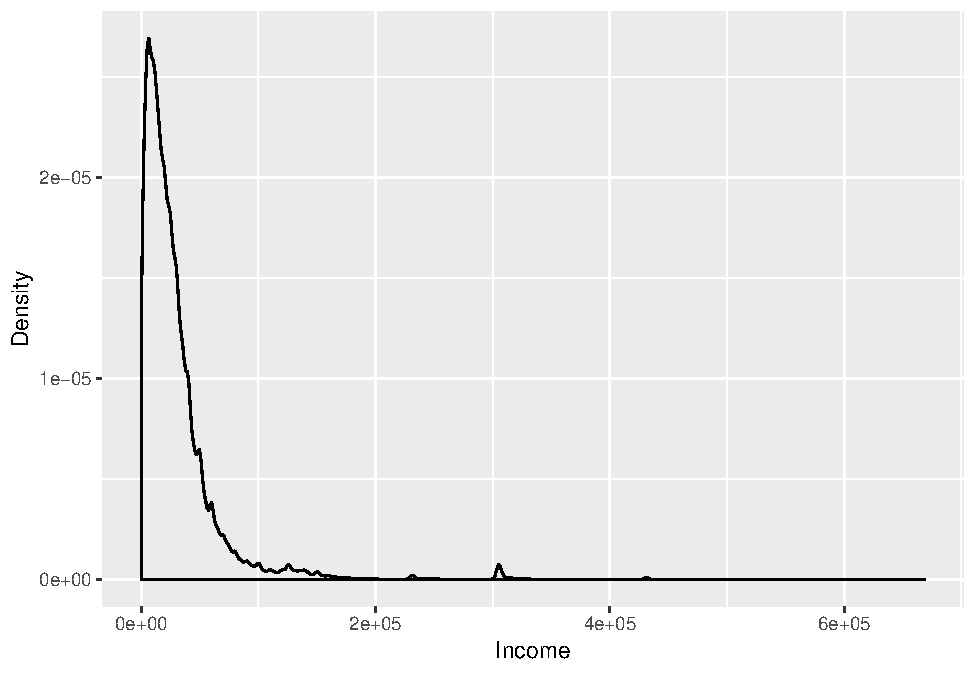
\includegraphics{Econometrics_using_R_files/figure-latex/unnamed-chunk-107-1.pdf}

\begin{itemize}
\tightlist
\item
  The distribution has a long tail.
\item
  Let's plot the distribution in \emph{log} scale
\end{itemize}

\begin{Shaded}
\begin{Highlighting}[]
\CommentTok{# `log` option specifies which axis is represented in log scale.}
\KeywordTok{qplot}\NormalTok{(pop, }\DataTypeTok{geom =} \StringTok{"density"}\NormalTok{, }
      \DataTypeTok{xlab =} \StringTok{"Income"}\NormalTok{,}
      \DataTypeTok{ylab =} \StringTok{"Density"}\NormalTok{,}
      \DataTypeTok{log =} \StringTok{"x"}\NormalTok{)}
\end{Highlighting}
\end{Shaded}

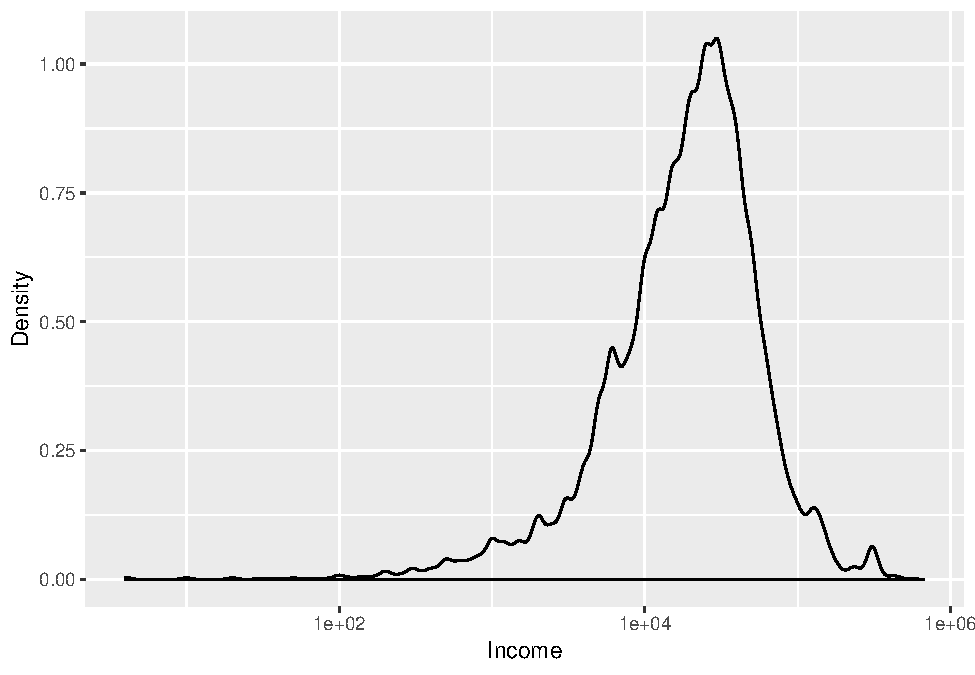
\includegraphics{Econometrics_using_R_files/figure-latex/unnamed-chunk-108-1.pdf}

\begin{itemize}
\tightlist
\item
  Let's investigate how close the sample mean constucted from the random
  sample is to the true population mean.
\item
  Step 1: Draw random sample\emph{s} from this population and calculate
  \(\bar{Y}\) for each sample.

  \begin{itemize}
  \tightlist
  \item
    Set the sample size \(N\).
  \end{itemize}
\item
  Step 2: Repeat 2000 times. You now have 2000 sample means.
\end{itemize}

\begin{Shaded}
\begin{Highlighting}[]
\CommentTok{# Set the seed for the random number. This is needed to maintaine the reproducibility of the results.}
\KeywordTok{set.seed}\NormalTok{(}\DecValTok{123}\NormalTok{)}

\CommentTok{# draw random sample of 100 observations from the variable pop}
\NormalTok{test <-}\StringTok{ }\KeywordTok{sample}\NormalTok{(}\DataTypeTok{x =}\NormalTok{ pop, }\DataTypeTok{size =} \DecValTok{100}\NormalTok{)}

\CommentTok{# Use loop to repeat 2000 times. }
\NormalTok{Nsamples =}\StringTok{ }\DecValTok{2000}
\NormalTok{result1 <-}\StringTok{ }\KeywordTok{numeric}\NormalTok{(Nsamples)}

\ControlFlowTok{for}\NormalTok{ (i }\ControlFlowTok{in} \DecValTok{1}\OperatorTok{:}\NormalTok{Nsamples )\{}
  
\NormalTok{  test <-}\StringTok{ }\KeywordTok{sample}\NormalTok{(}\DataTypeTok{x =}\NormalTok{ pop, }\DataTypeTok{size =} \DecValTok{100}\NormalTok{)}
\NormalTok{  result1[i] <-}\StringTok{ }\KeywordTok{mean}\NormalTok{(test)}
  
\NormalTok{\}}

\CommentTok{# Simple approach}
\NormalTok{result1 <-}\StringTok{ }\KeywordTok{replicate}\NormalTok{(}\DataTypeTok{expr =} \KeywordTok{mean}\NormalTok{(}\KeywordTok{sample}\NormalTok{(}\DataTypeTok{x =}\NormalTok{ pop, }\DataTypeTok{size =} \DecValTok{10}\NormalTok{)), }\DataTypeTok{n =}\NormalTok{ Nsamples)}
\NormalTok{result2 <-}\StringTok{ }\KeywordTok{replicate}\NormalTok{(}\DataTypeTok{expr =} \KeywordTok{mean}\NormalTok{(}\KeywordTok{sample}\NormalTok{(}\DataTypeTok{x =}\NormalTok{ pop, }\DataTypeTok{size =} \DecValTok{100}\NormalTok{)), }\DataTypeTok{n =}\NormalTok{ Nsamples)}
\NormalTok{result3 <-}\StringTok{ }\KeywordTok{replicate}\NormalTok{(}\DataTypeTok{expr =} \KeywordTok{mean}\NormalTok{(}\KeywordTok{sample}\NormalTok{(}\DataTypeTok{x =}\NormalTok{ pop, }\DataTypeTok{size =} \DecValTok{500}\NormalTok{)), }\DataTypeTok{n =}\NormalTok{ Nsamples)}

\CommentTok{# Create dataframe}

\NormalTok{result_data <-}\StringTok{ }\KeywordTok{data.frame}\NormalTok{(  }\DataTypeTok{Ybar10 =}\NormalTok{ result1, }
                            \DataTypeTok{Ybar100 =}\NormalTok{ result2, }
                            \DataTypeTok{Ybar500 =}\NormalTok{ result3)}
\end{Highlighting}
\end{Shaded}

\begin{itemize}
\tightlist
\item
  Step 3: See the distribution of those 2000 sample means.
\end{itemize}

\begin{Shaded}
\begin{Highlighting}[]
\CommentTok{# Use reshape library}
\CommentTok{# install.packages("reshape")}
\KeywordTok{library}\NormalTok{(}\StringTok{"reshape"}\NormalTok{)}

\CommentTok{# Use "melt" to change the format of result_data}
\NormalTok{data_for_plot <-}\StringTok{ }\KeywordTok{melt}\NormalTok{(}\DataTypeTok{data =}\NormalTok{ result_data, }\DataTypeTok{variable.name =} \StringTok{"Variable"}\NormalTok{ )}
\end{Highlighting}
\end{Shaded}

\begin{verbatim}
## Using  as id variables
\end{verbatim}

\begin{Shaded}
\begin{Highlighting}[]
\CommentTok{# Use "ggplot2" to create the figure.}
\CommentTok{# The variable `fig` contains the information about the figure}
\NormalTok{fig <-}\StringTok{ }
\StringTok{  }\KeywordTok{ggplot}\NormalTok{(}\DataTypeTok{data =}\NormalTok{ data_for_plot) }\OperatorTok{+}
\StringTok{  }\KeywordTok{xlab}\NormalTok{(}\StringTok{"Sample mean"}\NormalTok{) }\OperatorTok{+}\StringTok{ }
\StringTok{  }\KeywordTok{geom_line}\NormalTok{(}\KeywordTok{aes}\NormalTok{(}\DataTypeTok{x =}\NormalTok{ value, }\DataTypeTok{colour =}\NormalTok{ variable ),   }\DataTypeTok{stat =} \StringTok{"density"}\NormalTok{ ) }\OperatorTok{+}\StringTok{ }
\StringTok{  }\KeywordTok{geom_vline}\NormalTok{(}\DataTypeTok{xintercept=}\NormalTok{pop_mean ,}\DataTypeTok{colour=}\StringTok{"black"}\NormalTok{)}

\CommentTok{# Display the figure }
\KeywordTok{plot}\NormalTok{(fig)}
\end{Highlighting}
\end{Shaded}

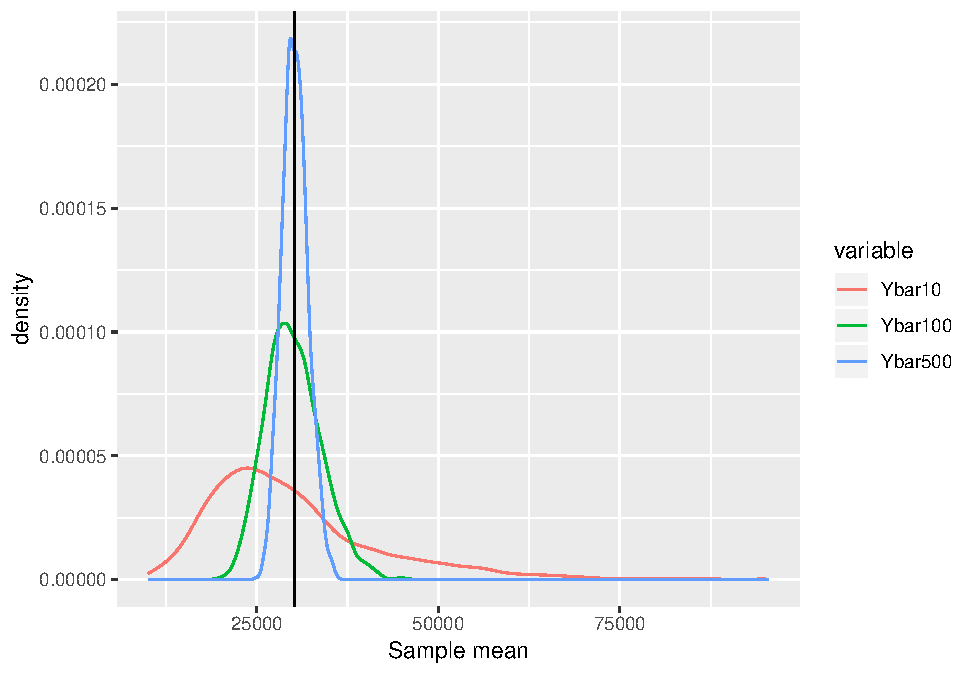
\includegraphics{Econometrics_using_R_files/figure-latex/unnamed-chunk-110-1.pdf}

\begin{itemize}
\tightlist
\item
  Observation 1: Regardless of the sample size, the average of the
  sample means is close to the population mean. \textbf{Unbiasdeness}
\item
  Observation 2: As the sample size gets larger, the distribution is
  concentrated around the population mean. \textbf{Consistency (law of
  large numbers)}
\end{itemize}

\section{Hypothesis Testing}\label{hypothesis-testing}

\subsection{Central limit theorem}\label{central-limit-theorem}

\begin{itemize}
\item
  Cental limit theorem: Consider the i.i.d. sample of
  \(Y_1,\cdots, Y_N\) drawn from the random variable \(Y\) with mean
  \(\mu\) and variance \(\sigma^2\). The following \(Z\) converges in
  distribution to the normal distribution. \[
  Z = \frac{1}{\sqrt{N}} \sum_{i=1}^N \frac{Y_i - \mu}{\sigma } \overset{d}{\rightarrow}N(0,1)
  \] In other words, \[
  \lim_{N\rightarrow\infty}P\left(Z \leq z\right)=\Phi(z)
  \]
\item
  The central limit theorem implies that if \(N\) is large
  \textbf{enough}, we can \textbf{approximate} the distribution of
  \(\bar{Y}\) by the standard normal distribution with mean \(\mu\) and
  variance \(\sigma^2 / N\) \textbf{regardless of the underlying
  distribution of \(Y\).}
\item
  Let's examine this property through simulation!!
\item
  Use the same example as before. Remember that the underlying income
  distribution is clearly NOT normal.

  \begin{itemize}
  \tightlist
  \item
    Population mean \(\mu = 30165.4673315\) and standard deviation
    \(\sigma = 38306.1712336\). Use these numbers.
  \end{itemize}
\end{itemize}

\begin{Shaded}
\begin{Highlighting}[]
\CommentTok{# Set the seed for the random number}
\KeywordTok{set.seed}\NormalTok{(}\DecValTok{124}\NormalTok{)}

\CommentTok{# define function for simulation }
\NormalTok{f_simu_CLT =}\StringTok{ }\ControlFlowTok{function}\NormalTok{(Nsamples, samplesize, pop, pop_mean, pop_sd )\{}
  
\NormalTok{  output =}\StringTok{ }\KeywordTok{numeric}\NormalTok{(Nsamples)}
  \ControlFlowTok{for}\NormalTok{ (i }\ControlFlowTok{in} \DecValTok{1}\OperatorTok{:}\NormalTok{Nsamples )\{}
\NormalTok{    test <-}\StringTok{ }\KeywordTok{sample}\NormalTok{(}\DataTypeTok{x =}\NormalTok{ pop, }\DataTypeTok{size =}\NormalTok{ samplesize)}
\NormalTok{    output[i] <-}\StringTok{ }\NormalTok{( }\KeywordTok{mean}\NormalTok{(test) }\OperatorTok{-}\StringTok{ }\NormalTok{pop_mean ) }\OperatorTok{/}\StringTok{ }\NormalTok{(pop_sd }\OperatorTok{/}\StringTok{ }\KeywordTok{sqrt}\NormalTok{(samplesize))}
\NormalTok{  \}}
  
  \KeywordTok{return}\NormalTok{(output)}

\NormalTok{\}}

\CommentTok{# Comment: You can do better without using forloop. Let me know if you come with a good idea.}

\CommentTok{# Run simulation }
\NormalTok{Nsamples =}\StringTok{ }\DecValTok{2000}
\NormalTok{result_CLT1 <-}\StringTok{ }\KeywordTok{f_simu_CLT}\NormalTok{(Nsamples, }\DecValTok{10}\NormalTok{, pop, pop_mean, pop_sd )}
\NormalTok{result_CLT2 <-}\StringTok{ }\KeywordTok{f_simu_CLT}\NormalTok{(Nsamples, }\DecValTok{100}\NormalTok{, pop, pop_mean, pop_sd )}
\NormalTok{result_CLT3 <-}\StringTok{ }\KeywordTok{f_simu_CLT}\NormalTok{(Nsamples, }\DecValTok{1000}\NormalTok{, pop, pop_mean, pop_sd )}

\CommentTok{# Random draw from standard normal distribution as comparison}
\NormalTok{result_stdnorm =}\StringTok{ }\KeywordTok{rnorm}\NormalTok{(Nsamples)}

\CommentTok{# Create dataframe}
\NormalTok{result_CLT_data <-}\StringTok{ }\KeywordTok{data.frame}\NormalTok{(  }\DataTypeTok{Ybar_standardized_10 =}\NormalTok{ result_CLT1, }
                            \DataTypeTok{Ybar_standardized_100 =}\NormalTok{ result_CLT2, }
                            \DataTypeTok{Ybar_standardized_1000 =}\NormalTok{ result_CLT3, }
                            \DataTypeTok{Standard_Normal =}\NormalTok{ result_stdnorm)}

\CommentTok{# Note: If you wanna quicky plot the density, type `plot(density(result1))`. }
\end{Highlighting}
\end{Shaded}

\begin{itemize}
\tightlist
\item
  Now take a look at the distribution.
\end{itemize}

\begin{Shaded}
\begin{Highlighting}[]
\CommentTok{# Use "melt" to change the format of result_data}
\NormalTok{data_for_plot <-}\StringTok{ }\KeywordTok{melt}\NormalTok{(}\DataTypeTok{data =}\NormalTok{ result_CLT_data, }\DataTypeTok{variable.name =} \StringTok{"Variable"}\NormalTok{ )}
\end{Highlighting}
\end{Shaded}

\begin{verbatim}
## Using  as id variables
\end{verbatim}

\begin{Shaded}
\begin{Highlighting}[]
\CommentTok{# Use "ggplot2" to create the figure.}
\NormalTok{fig <-}\StringTok{ }
\StringTok{  }\KeywordTok{ggplot}\NormalTok{(}\DataTypeTok{data =}\NormalTok{ data_for_plot) }\OperatorTok{+}
\StringTok{  }\KeywordTok{xlab}\NormalTok{(}\StringTok{"Sample mean"}\NormalTok{) }\OperatorTok{+}\StringTok{ }
\StringTok{  }\KeywordTok{geom_line}\NormalTok{(}\KeywordTok{aes}\NormalTok{(}\DataTypeTok{x =}\NormalTok{ value, }\DataTypeTok{colour =}\NormalTok{ variable ),   }\DataTypeTok{stat =} \StringTok{"density"}\NormalTok{ ) }\OperatorTok{+}\StringTok{ }
\StringTok{  }\KeywordTok{geom_vline}\NormalTok{(}\DataTypeTok{xintercept=}\DecValTok{0}\NormalTok{ ,}\DataTypeTok{colour=}\StringTok{"black"}\NormalTok{)}

\KeywordTok{plot}\NormalTok{(fig)}
\end{Highlighting}
\end{Shaded}

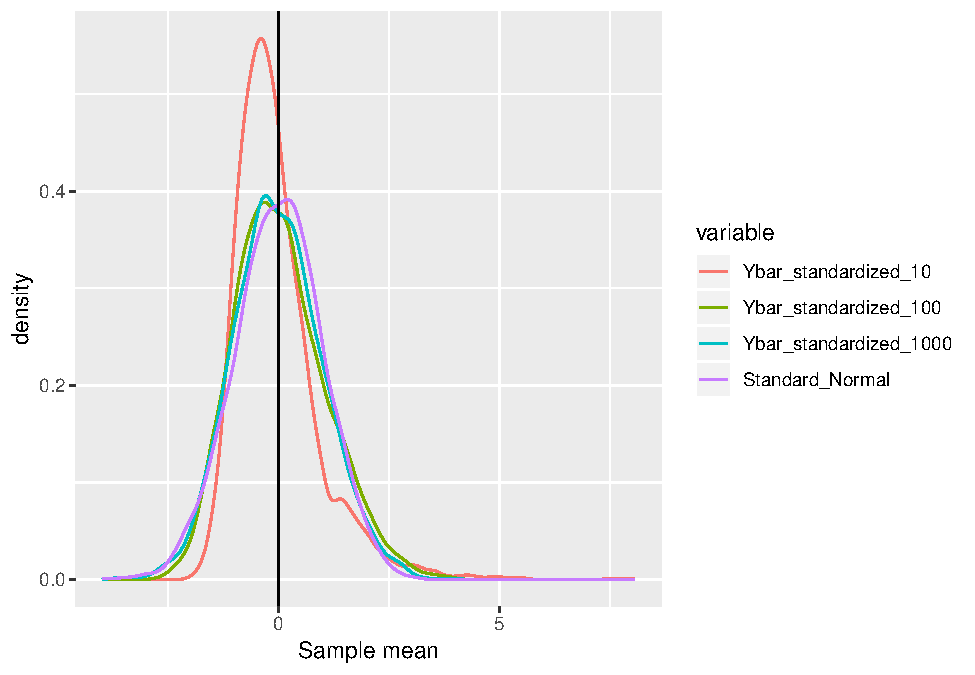
\includegraphics{Econometrics_using_R_files/figure-latex/unnamed-chunk-112-1.pdf}

\begin{itemize}
\tightlist
\item
  As the sample size grows, the distribution of \(Z\) converges to the
  standard normal distribution.
\end{itemize}

\subsection{Hypothesis testing}\label{hypothesis-testing-1}

To be added.


\end{document}
